\documentclass[12pt, a4paper]{report}

\usepackage[utf8]{inputenc}
\usepackage[T1]{fontenc}
\usepackage{times}
\usepackage{geometry}
\usepackage{graphicx}
\usepackage{xcolor}
\usepackage{setspace}
\usepackage{titlesec}
\usepackage{fancyhdr}
\usepackage{hyperref}
\usepackage{booktabs}
\usepackage{amsmath}
\usepackage{amsfonts}
\usepackage{amssymb}
\usepackage{array}
\usepackage{multirow}
\usepackage{caption}
\usepackage{tocloft}
\usepackage{pifont}
\usepackage{tabularx}
\usepackage{adjustbox}
\usepackage{float}
\usepackage{cite}

\geometry{
    top=1.0in,
    bottom=1.0in,
    left=1.25in,
    right=1.0in
}

\hypersetup{
    colorlinks=true,
    linkcolor=black,
    citecolor=black,
    urlcolor=blue
}

\onehalfspacing

% Optimized chapter and section spacing for publication quality (~45 pages target)
\titleformat{\chapter}[display]
  {\normalfont\Large\bfseries}{Chapter \thechapter}{8pt}{\LARGE}
\titlespacing*{\chapter}{0pt}{-10pt}{14pt}
\titlespacing*{\section}{0pt}{10pt}{4pt}
\titlespacing*{\subsection}{0pt}{8pt}{3pt}

\captionsetup{font=small, labelfont=bf, skip=6pt}

\pagestyle{fancy}
\setlength{\headheight}{14.5pt}
\fancyhf{}
\fancyhead[L]{\leftmark}
\fancyhead[R]{\thepage}
\renewcommand{\headrulewidth}{0.4pt}

\begin{document}

% =========================================================================
% TITLE PAGE
% =========================================================================
\begin{titlepage}
    \centering
    \vspace*{0.3cm}

    {\LARGE \textbf{
A Closed-Loop Wearable EEG Framework\\[0.3cm]
for Migraine Mitigation\\[0.3cm]
via Binaural Beat Entrainment
}}\\[1.5cm]

    {\large \textbf{By}}\\[0.3cm]
    {\large Abu Hurayra Mahbe -- 0112230043}\\
    {\large Md. Shakibul Hassan Prince -- 0112230048}\\
    {\large Jarin Tabassum -- 0112230836}\\
    {\large Anisa Azmi -- 0112230292}\\
    {\large Mahmudul Mashrafe -- 0112230115}\\[1.5cm]

    {\large Submitted in partial fulfilment of the requirements of the\\ degree of Bachelor of Science in Computer Science and Engineering}\\[1.5cm]

    {\large June 11, 2026}\\[1.2cm]

    \IfFileExists{Images/uiu_logo.png}{%
        
\includegraphics[width=0.22\textwidth]{Images/uiu_logo.png}\\[0.4cm]
    }{%
        \vspace{1.2cm}
    }
    {\large Department of Computer Science and Engineering\\
    United International University}

    \vfill
\end{titlepage}

\pagenumbering{roman}

% =========================================================================
% ABSTRACT
% =========================================================================
\chapter*{Abstract}
\addcontentsline{toc}{chapter}{Abstract}
Migraine is a debilitating chronic neurovascular disorder that affects over one billion people globally. It is characterised by Thalamo-Cortical Dysrhythmia (TCD), increased cortical excitability, and sensory habituation anomalies. These can often lead to unwanted side effects, medication overuse headaches, and poor compliance with conventional medication. This Final Year Design Project provides an integrated neuro-engineering approach to migraine treatment using EEG Time-Frequency Classification and neuromodulation using tailored sound. A pipeline was developed to preprocess the data taken from the Carnegie Mellon University (CMU) ultra-high density dataset. It contained 128-channel EEG recordings from resting state and sensory stimuli (Auditory SSAEP \& Visual SSVEP). The data was preprocessed using Common Average Referencing (CAR), Bandpass Filtering (1.0--50.0 Hz) and Notch Filtering (60 Hz). The data from the occipital channel (\#80) was transformed into time-frequency spectrograms using a Short-Time Fourier Transform (STFT). The spectrograms were created using a Viridis Colourmap and had a dynamic range of $[-10, +30]$ dB. We then used three different models to classify the data: VGG16, ResNet50 and EfficientNetB7. EfficientNetB7 gave the best results, with an accuracy of 93.75\%, weighted precision of 94.71\%, weighted F1 Score of 93.85\% and MCC of 0.8750. In comparison, VGG16 had an accuracy of 90.63\% and MCC of 0.7985, whilst ResNet50 had an accuracy of 87.50\% and MCC of 0.7410. An algorithm was developed to analyse the RGB Colourmap. Each pixel's RGB value was matched to its nearest colour in the 256-colour Viridis LUT using least Euclidean distance. This allowed an approximate power spectral density ($\mu\text{V}^2/\text{Hz}$) to be extracted from the spectrogram. This provided a way of finding patient-specific electrophysiological information such as individual alpha frequency (IAF), alpha deficit (relative alpha power below a 20\% reference) and Theta to Alpha Ratio (TAR). In a descriptive analysis of resting-state participants (12 migraine, 22 control), relative theta power was slightly higher in migraine patients ($15.47 \pm 8.48\%$ vs $13.17 \pm 5.93\%$), whereas relative alpha power and TAR did not show the group-level alpha reduction reported in the literature; no statistical tests were performed. Using the individual alpha frequency, a sound generator was used to create customised binaural beats from dual pure tones. These were centred around a carrier frequency of 216 Hz. The beats had a squared half-cosine taper of 1.5 seconds to avoid clicking. An example patient (M10) was analysed and had an alpha frequency peak detected at 10.09 Hz. The algorithm also detected an alpha deficit of 7.88\%. A beat was then generated with a precise frequency of 10.09 Hz ($f_{\text{left}} = 210.96$ Hz and $f_{\text{right}} = 221.05$ Hz). The beat was stored as a stereo 16-bit audio file at a sampling frequency of 44.1 kHz. This project creates a technology that allows Deep Neural Networks to be used to detect migraine and create tailored sound to target the auditory cortex. This provides a proof-of-concept software pipeline towards a scalable digital solution for migraine; clinical efficacy has not yet been tested.
\newpage

% =========================================================================
% ACKNOWLEDGEMENTS
% =========================================================================
\chapter*{Acknowledgements}
\addcontentsline{toc}{chapter}{Acknowledgements}
We express our deepest gratitude to our project supervisor, \textbf{Dr.~Jannatun Noor Mukta}, for her guidance, academic critique, and continuous encouragement throughout this Final Year Design Project. Her insights into biomedical signal processing and machine learning have shaped the foundation of this work.

We extend our sincere thanks to \textbf{RA Md Abu Obaida Zishan}, our laboratory coordinator, for his technical assistance, practical troubleshooting suggestions, and feedback on algorithmic pipelines. We also express our respect to \textbf{Dr.~Hasan Sarwar}, Head of the Department of Computer Science and Engineering at United International University, and the faculty for providing high-performance computing infrastructure and academic resources.

We are deeply appreciative of the authors of the open-access CMU Ultra-High-Density EEG dataset---Dr.~Alireza Chamanzar, Dr.~Sarah M. Haigh, Dr.~Pulkit Grover, and Dr.~Marlene Behrmann---whose experimental work provided the empirical foundation for our investigations. Finally, we thank our families and teammates for their dedication and support throughout this endeavor.

\newpage

% =========================================================================
% PUBLICATION LIST
% =========================================================================
\chapter*{Publication List}
\addcontentsline{toc}{chapter}{Publication List}

\subsection*{Journal Articles (Prepared / Under Submission)}
\begin{enumerate}
    \item \textbf{A. H. Mahbe, M. S. H. Prince, J. Tabassum, A. Azmi, M. Mashrafe, and J. N. Mukta}, ``Spectrogram-Driven Deep Transfer Learning and Analytical Colormap Inversion for Personalized Binaural Beat Neuromodulation in Interictal Migraine,'' target venue: \textit{IEEE Transactions on Neural Systems and Rehabilitation Engineering} / \textit{Biomedical Signal Processing and Control}, 2026.
\end{enumerate}

\subsection*{Conference Papers (Prepared / Under Submission)}
\begin{enumerate}
    \item \textbf{M. Mashrafe, A. H. Mahbe, M. S. H. Prince, J. Tabassum, A. Azmi, and J. N. Mukta}, ``A Closed-Loop Framework for Interictal Migraine Classification via Convolutional Neural Networks and Individual Alpha Frequency Acoustic Entrainment,'' target venue: \textit{IEEE International Conference on Biomedical and Health Informatics (BHI)}, 2026.
\end{enumerate}

\subsection*{Open-Source Deliverables and Data Artifacts}
\begin{enumerate}
    \item \textbf{FYDP-III Research Artifacts}: Complete Jupyter Notebook repository comprising raw EEG preprocessing (\texttt{1\_EEG\_CMU.ipynb}), deep transfer learning benchmarks (\texttt{2\_Migraine\_VGG16\_Spectrogram.ipynb}, \texttt{3\_Migraine\_EfficientNetB7\_Spectrogram.ipynb}, \texttt{4\_Migraine\_ResNet50\_Spectrogram.ipynb}), and the spectrogram inversion audio synthesis engine (\texttt{5\_spectrogram\_binaural\_treatment.ipynb}).
    \item \textbf{Audio Prescription Repository}: Cohort-wide synthesized 16-bit 44.1~kHz stereo WAV binaural beat prescriptions tailored to individual alpha frequencies across all migraine subjects.
\end{enumerate}

\newpage

% =========================================================================
% TABLE OF CONTENTS & LISTS
% =========================================================================
\tableofcontents
\newpage

\listoffigures
\addcontentsline{toc}{chapter}{List of Figures}
\newpage

\listoftables
\addcontentsline{toc}{chapter}{List of Tables}
\newpage

% =========================================================================
% CHAPTER 1: INTRODUCTION
% =========================================================================
\pagenumbering{arabic}
\chapter{Introduction}
\label{ch:introduction}

\section{Project Overview}
\label{sec:project_overview}
Migraine is an intensely debilitating chronic neurological disorder characterized by recurrent episodes of severe throbbing headache, typically unilateral, accompanied by autonomic and sensory disturbances including nausea, photophobia, and phonophobia \cite{Zhang2023,VanDenHoek2024}. In approximately one-third of sufferers, attacks are preceded by focal neurological aura symptoms \cite{Riederer2023}. According to the Global Burden of Disease (GBD) studies, migraine ranks among the leading causes of years lived with disability (YLD) globally, affecting over 1.1 billion individuals with disproportionate prevalence in working-age adults \cite{Petrusic2025,DanelakisStubberud2025}.

Despite its societal toll, clinical management remains dominated by acute analgesics (triptans, NSAIDs) and preventive medications (beta-blockers, topiramate, CGRP antagonists) \cite{Quartetti2025,Shamsi2024}. However, over 40\% of patients report unsatisfactory relief, debilitating side effects, or contraindications \cite{Shamsi2024}. Moreover, frequent acute medication intake frequently causes medication overuse headache (MOH), transforming episodic migraine into intractable chronic states \cite{GomezPilar2022}. Hence, there is an urgent demand for non-invasive, non-pharmacological digital therapeutics capable of objective detection and patient-tailored intervention.

Quantitative electroencephalography (qEEG) reveals that migraineurs exhibit significant neurophysiological disturbances during interictal (headache-free) periods, prominently \textit{thalamocortical dysrhythmia} (TCD) and pervasive cortical hyperexcitability \cite{VanDenHoek2024,AbdulhusseinAldeen2024}. These abnormalities manifest as altered spectral power distributions, lack of habituation to repetitive visual/auditory stimuli, and marked suppression of posterior alpha oscillations (8.0--13.0~Hz) \cite{chamanzar2021uhd,Zhang2023,FrimpongManson2024}. Concurrently, acoustic neuromodulation using \textit{binaural beats} has emerged as a promising non-invasive mechanism to modulate cortical rhythms via the auditory frequency-following response (FFR) in the brainstem \cite{Oster1973,Wahbeh2007,Ingendoh2023}.

However, existing research remains fragmented. Diagnostic studies focus on offline machine learning classification without therapeutic intervention \cite{aslan2023migrainecnn,orhanbulucu2023hybrid}, while commercial binaural beat applications deliver generic, fixed-frequency audio (e.g., standard 10~Hz) that ignores patient-specific Individual Alpha Frequency (IAF) and power deficits \cite{CoronaGonzalez2021,KahathuduwaBlume2025}. This Final Year Design Project bridges this gap by introducing an end-to-end software framework that couples deep learning-based interictal migraine detection from 2D STFT spectrograms with an analytical colormap inversion algorithm that extracts patient-specific IAF values to synthesize customized binaural beat audio prescriptions. Here, ``closed-loop'' refers to the automated chain from detection to personalized prescription; real-time, sensor-in-the-loop feedback is left for future work.

\section{Motivation and Objectives}
\label{sec:motivation_objectives}
This research addresses both clinical necessities and computational engineering opportunities:
\begin{itemize}
    \item \textbf{Non-Pharmacological Therapy}: Exploring a potentially side-effect-free alternative to pharmaceutical prophylaxis that aims to restore cortical oscillatory balance \cite{Quartetti2025,Shamsi2024}.
    \item \textbf{Objective Biomarker Diagnostics}: Replacing subjective clinical recall with objective qEEG signatures of cortical hyperexcitability and thalamocortical slowing \cite{chamanzar2021uhd,Petrusic2025}.
    \item \textbf{Time-Frequency Computer Vision}: Exploiting 2D time-frequency spectrogram representations to utilize pre-trained deep convolutional networks (CNNs) for robust feature extraction \cite{orhanbulucu2023hybrid,Rakhmatulin2024}.
    \item \textbf{Patient-Specific Resonant Entrainment}: Tailoring binaural beat frequencies to each patient's intrinsic IAF, with the aim of maximizing auditory-cortical phase-locking \cite{Melnichuk2025,Hamid2025,alonso2024individualized}.
\end{itemize}

The specific project objectives are:
\begin{enumerate}
    \item Implement a standardized biomedical preprocessing pipeline for 128-channel ultra-high-density EEG (CAR, 1.0--50.0~Hz FIR bandpass, 60~Hz notch filtering).
    \item Generate 2D STFT spectrogram images from visual/occipital channel recordings across resting-state, SSAEP, and SSVEP paradigms.
    \item Train and benchmark deep transfer learning models (VGG16, ResNet50, EfficientNetB7) for automated interictal migraine detection.
    \item Formulate an analytical RGB colormap inversion algorithm converting pixel intensities into approximate linear power spectral density ($\mu\text{V}^2/\text{Hz}$).
    \item Extract patient-specific IAF, Alpha Deficits, and Theta-to-Alpha Ratios (TAR).
    \item Engineer a digital audio synthesis engine generating click-free dichotic stereo binaural beat prescriptions modulated to each patient's IAF.
    \item Evaluate the complete framework through population cohort analytics and single-subject case studies.
\end{enumerate}

\section{Organization of the Report}
\label{sec:organization}
The remainder of this report is organized as follows: Chapter~\ref{ch:background} presents neurophysiological preliminaries, a structured five-domain literature review, and comprehensive research gap analysis. Chapter~\ref{ch:project_design} details the end-to-end methodology, dataset architecture, signal preprocessing, deep transfer learning models, analytical colormap inversion, and binaural audio synthesis. Chapter~\ref{ch:experimental_results} presents empirical classification results, confusion matrices, ROC curves, the patient M10 case study, and cohort analytics. Chapter~\ref{ch:design_constraints} evaluates engineering standards, acoustic safety, and design constraints. Chapter~\ref{ch:conclusion} concludes with principal findings, limitations, and future research directions.

% =========================================================================
% CHAPTER 2: BACKGROUND & LITERATURE REVIEW
% =========================================================================
\chapter{Background and Literature Review}
\label{ch:background}

\section{Neurophysiological Foundations of Migraine}
\label{sec:neuro_foundations}
Migraine pathophysiology involves complex neurovascular dysfunction characterized by recurrent trigeminovascular activation, cortical spreading depression (CSD), and abnormal sensory modulation \cite{Zhang2023,VanDenHoek2024}. A hallmark of the interictal migraine brain is \textit{thalamocortical dysrhythmia} (TCD) \cite{VanDenHoek2024,AbdulhusseinAldeen2024}. In healthy neural circuits, the thalamus acts as a sensory gate, filtering afferent information and pacing cortical networks via rhythmic alpha oscillations (8.0--13.0~Hz) generated through reciprocal thalamic reticular nucleus interactions \cite{Zhang2023}. In migraine, de-inactivation of low-threshold T-type calcium channels is thought to induce low-frequency thalamic burst firing in the theta band (4.0--8.0~Hz), causing disruption of thalamocortical pacing, reduction of posterior alpha power, and unmasking of cortical hyperexcitability.

A defining electrophysiological consequence of TCD is the \textit{lack of habituation} to repetitive sensory stimuli \cite{chamanzar2021uhd,AbdulhusseinAldeen2024}. Whereas healthy brains exhibit decreased evoked potential amplitudes during sustained visual or auditory stimulation, migraineurs display deficient habituation or sensory potentiation, indicating abnormal sensory gating and cortical hyperexcitability.

\section{Principles of Binaural Beat Neuromodulation}
\label{sec:binaural_principles}
Binaural beats are auditory illusions perceived when two pure tones of slightly differing frequencies ($f_1$ and $f_2$) are delivered dichotically to each ear through stereo headphones \cite{Oster1973}. The acoustic signals converge in the brainstem at the \textit{medial superior olive} (MSO) of the superior olivary complex (SOC), the primary structure responsible for sound localization via interaural phase differences (IPD) \cite{Wahbeh2007}. The cyclic phase disparity causes MSO neurons to discharge action potentials phase-locked to the difference frequency:
\begin{equation}
    f_{\text{beat}} = |f_1 - f_2|
    \label{eq:binaural_beat_freq}
\end{equation}
This phase-locked neural activity ascends through the lateral lemniscus and inferior colliculus to the medial geniculate body of the thalamus and auditory cortex, generating a \textit{frequency-following response} (FFR) \cite{Ingendoh2023,Shamsi2024}. When tuned to the alpha range ($f_{\text{beat}} \in [8.0, 13.0]$~Hz), binaural beats are hypothesised to drive resonant thalamocortical synchronization, restoring sensory gating and mitigating cortical hyperexcitability \cite{CoronaGonzalez2021,Melnichuk2025,magalhaes2025auditory}; direct clinical evidence in migraine remains limited.

\section{Structured Literature Review}
\label{sec:literature_review}
To establish the context of our contributions, existing literature was reviewed across five distinct domains: (1) EEG and Biomarkers for Migraine, (2) Binaural Beats and Brainwave Entrainment, (3) Wearable EEG Platforms and Digital Phenotyping, (4) Feature Extraction and Machine Learning Approaches, and (5) Binaural Beat Generation and Acoustic Neuromodulation Systems.

\subsection{Domain 1: EEG and Biomarkers for Migraine}
\label{subsec:lit_eeg_biomarkers}
For the past several decades, researchers have studied the role of EEG as a biomarker for migraine disease. Initial studies demonstrated that delta/theta activity was higher during migraine attacks and beta was higher between attacks. Newer studies that have used the quantitative EEG (qEEG) method confirm evidence of cortical hyperexcitability among people who suffer from migraines, including decreased alpha activity, high-frequency oscillations, and interhemispheric coherence abnormalities \cite{VanDenHoek2024}. Magnetoencephalography (MEG) studies localized the areas of cortical hyperexcitability to occipital, parietal, and prefrontal cortices, which are related to sensory perception and pain processing. Notably, investigators determined that quantitative EEG alterations occurred up to 36 hours pre-migraine and could thus be used as a prodromal biomarker \cite{Kim2023}.

The study conducted by Joshi et al.~\cite{JoshiMatharu2025} used EEG to create spiking and convolutional spiking neural networks (CSNN) to detect stress with an emphasis on developing temporal models that would provide accurate predictions while minimizing energy consumption; their convolutional spiking neural network achieved 98.61\% accuracy, 100\% sensitivity, and 98.60\% F1-score, demonstrating rapid processing speed and compactness for use with wearable devices. Van den Hoek et al.~\cite{VanDenHoek2024} offered an overview of spontaneous EEG, evoked potentials, and treatment-related alterations throughout the migraine cycle to assess EEG as a marker of susceptibility, wherein preictal alterations in theta/alpha power, slowing, and connectivity were found to be consistently present, but no single secure marker was discovered; it was determined that future duties will include using home-based wearable EEG devices and implementing conventional protocols to study biomarker susceptibility to migraine.

Zhang and colleagues~\cite{Zhang2023} evaluated EEG use in migraine (i.e., resting and stimulus-evoked spectral characteristics, connectivity, microstates, and machine learning/deep learning classifiers), reporting previously seen changes (i.e., greater alpha slowing, elevated delta/theta, modified networks, and the presence of useful ML classifiers) alongside logistical challenges (i.e., individual variance and small participant numbers) when defining reliable biomarkers. Analyzing EEG data, Frimpong-Manson et al.~\cite{FrimpongManson2024} used both prospective and retrospective data from large-sized cohorts to identify objective migraine signatures and described interictal (period of no migraine) increased occipital 12--13~Hz power as reproducible headache biomarkers. They demonstrated that their KNN and SVM machine learning algorithms classified migraines and controls with 87.2\% accuracy, supporting the use of occipital alpha as a headache biomarker candidate.

Quartetti et al.~\cite{Quartetti2025} conducted a systematic review of 36 studies identifying lifestyle factors incident to episodic migraines to develop forecasting algorithms. They concluded that ketogenic diets, supplements, and physical activity are evidence-based strategies to reduce the number of attacks and could be used to generate predictive models; however, no EEG headache biomarkers or machine learning models have been directly tested. Additionally, Zebhauser et al.~\cite{Zebhauser2024}, in their meta-analysis of 27 studies using EEG/MEG techniques of individuals with migraine, found a candidate EEG signature for migraine based upon increased theta power and reduced alpha-to-beta connectivity between brain regions to measure presymptomatic migraine; they noted that these findings had significant methodological limitations including presence of comorbidities, small sample sizes, and differential methodologies.

Findings on Steady-State Visual Evoked Potentials (SSVEPs) by Abdulhussein et al.~\cite{AbdulhusseinAldeen2024} suggest that rhythmic sensory stimulation can act as a pacemaker for thalamocortical dysrhythmias in migraine. In their systematic review, Gomez-Pilar et al.~\cite{GomezPilar2022} also found that EEG, MRI, and PET imaging studies provide evidence of different brain network activity patterns between individuals with chronic and episodic migraine. Consistent differences in fast EEG/MEG bands and in networks involved in pain processing and emotional responses were identified, suggesting that functional multimodal biomarkers may provide objective markers for determining whether an individual is at higher risk for developing chronic migraine.

Riederer et al.~\cite{Riederer2023} published a narrative review of the EEG and MRI characteristics of migraine aura in order to assist neurologists in differential diagnosis: typically, uncomplicated visual auras show normal scalp EEG, whereas complex auras typically show focal slowing or suppression of acute phase EEG, providing possible differentiators between migraine aura and stroke or epileptic seizures. Göker~\cite{Goker2023} proposed a novel automated migraine detection system using Welch's method (1.0--49.0~Hz) and reported that a 128-channel BiLSTM achieved an overall accuracy of 95.99\%, with a sensitivity of 0.96, a specificity of 0.95, and an F1 score of 0.96, outperforming RF, SVM, and LDA classifiers trained on the same EEG dataset.

Kedgan et al.~\cite{Kedgan2025} conducted a systematic review and pooled prevalence meta-analysis of EEG patterns at the different phases of aura, headache, post-headache, and interictal states for hemiplegic migraine. They found low-amplitude, contralateral background activity during the aura phase, followed by focal slowing of the EEG during the headache phase, with largely normal EEG during the interictal phase alongside evidence of genotype-related differences. A scoping review on EEG for diagnosing and classifying migraines was presented by Raghuraman and Joshi~\cite{RaghuramanJoshi2024}, who found evidence of cortical hyperexcitability, deficits in habituation, abnormal microstates (decreased class C, increased class B/D microstates), and automated AR-Burg models (up to 88.7\% accuracy); however, they concluded that methodological heterogeneity and a current focus on migraine without aura prevent the establishment of a reliable automated etiology-based diagnostic system. An evaluation of qEEG as a potential biomarker of migraine was performed by Kim et al.~\cite{Kim2023}, who evaluated 720 subjects using z-score maps and found that individuals with migraines demonstrated an elevated level of overall absolute power compared to individuals without migraines, with particularly high levels of absolute power in the beta frequency range (25--30~Hz), correlating with clinical improvement and supporting the diagnostic utility of qEEG.

\subsection{Domain 2: Binaural Beats and Brainwave Entrainment}
\label{subsec:lit_binaural_beats}
Melnichuk et al.~\cite{Melnichuk2025} employed a sustained attention Continuous Performance Task (CPT) with parametric variations of beta (16~Hz) and gamma (40~Hz) binaural beats. EEG entrainment was reliable, especially for gamma binaural beats, and a small improvement in hit rate was observed under optimal acoustic conditions (40~Hz beat, 340~Hz carrier, white noise masking, task-onset delivery). Yang et al.~\cite{Yang2025} conducted a randomized crossover study of 6, 10, and 25~Hz binaural beats in college students. All binaural beat configurations reduced heart rate and blood pressure, while 25~Hz produced the strongest parasympathetic shift (normalized low-frequency power decreased, normalized high-frequency power increased), although EEG measurements were omitted.

Xiong et al.~\cite{Xiong2025} performed a meta-analysis of 15 randomized controlled trials (RCTs) of binaural beats in the perioperative period. Anxiety reduction was substantial (Standardized Mean Difference [SMD] $-1.0$ to $-1.4$) alongside moderate pain relief and hemodynamic stabilization compared to silence or non-binaural beat audio control conditions. Kahathuduwa et al.~\cite{KahathuduwaBlume2025} engineered real-time EEG-guided binaural beats and demonstrated enhanced relaxation and cognitive performance compared to controls, verifying the validity of adaptive, closed-loop acoustic entrainment. Shamsi et al.~\cite{Shamsi2024} performed a systematic review of binaural beats in pain management, reporting that alpha and delta-alpha binaural beats are effective in acute procedural pain, whereas results in chronic pain remain heterogeneous due to methodological variability.

By using wearable EEG to compare stationary binaural beats, panning sounds, and pure-tone beeps, Sudre et al.~\cite{Sudre2024} demonstrated that spatial acoustic motion produced stronger relaxation and cortical modulation than static beat illusions alone. Ingendoh et al.~\cite{Ingendoh2023} examined 14 EEG studies and concluded that only 5 demonstrated statistically verifiable entrainment (none convincingly in the beta band), recommending that standardized stimulus protocols be established before making broad generalizations. In their study of 0.25~Hz and 1.0~Hz beats during daytime naps, Fan et al.~\cite{Fan2024} found that 0.25~Hz stimulation shortens N2/N3 slow-wave sleep onset latency without overwhelming phase-locking, indicating behavioral slow-wave facilitation.

Binaural beats were tested during cadaveric dissection by Mosheshe et al.~\cite{Mosheshe2024}, who found that acoustic stimulation helped students cope with acute emotional stress and significantly decreased subjective anxiety compared to silent controls. Chockboondee et al.~\cite{ChockboondeeJatupornpoonsub2023} investigated long versus short beat exposure durations, finding that extended sessions significantly reduced heart rate and the LF/HF ratio while improving mood scores measured via Brunel Mood Scale (BRUMS), demonstrating dose-dependent relaxation effects. Dabiri et al.~\cite{Dabiri2022} showed that delta beats enhanced sleep quality and post-sleep mood among pilot subjects, supporting auditory sleep aids pending further electrophysiological validation.

According to Corona-González et al.~\cite{CoronaGonzalez2021}, customized theta and beta beats increased target spectral power significantly more than rigid, fixed-frequency beats, emphasizing the necessity of individual tuning. Al-Shargie et al.~\cite{AlShargie2022} utilized functional near-infrared spectroscopy (fNIRS) and 16~Hz binaural beats during Stroop tasks, documenting a 44\% reduction in salivary alpha-amylase stress biomarkers alongside heightened prefrontal activation and enhanced response speed. Wang et al.~\cite{WangZhang2022} observed that 40~Hz binaural beats increased gamma and alpha power while suppressing delta activity, yielding improved working memory capacity. A meta-analysis of binaural beats in cognition by Basu and Banerjee~\cite{BasuBanerjee2023} showed small but statistically significant improvements in memory and attention. Furthermore, Hamid et al.~\cite{Hamid2025} verified that alpha binaural beats specifically activated parietal-occipital EEG rhythms and cognitive processing compared to white noise controls.

\subsection{Domain 3: Wearable EEG Platforms and Digital Phenotyping}
\label{subsec:lit_wearable_systems}
Petru\v{s}i\'{c}~\cite{Petrusic2025} characterized EEG-based brain--computer interface (BCI) technology as an emerging, scalable solution for brain monitoring and assistive rehabilitation, enabling real-world neural signal acquisition without the clinical risks of invasive systems. They categorized wearable EEG systems into scalp-EEG, forehead-EEG, and ear-EEG topologies, noting that scalp-EEG systems achieve motor imagery and cognitive classification accuracies of 90--96\%. However, Petru\v{s}i\'{c} underscored critical challenges, including high susceptibility to motion artifacts, inter-subject variability, electrode impedance instability, and the absence of standardized benchmarking frameworks.

He et al.~\cite{He2023} conducted an exhaustive evaluation of commercial wireless EEG systems, showing that contemporary hardware remains highly heterogeneous with respect to channel count, sampling rates, battery life, and pricing (ranging from \$240 to \$30{,}000). While this diversity reflects rapid innovation, He et al. emphasized the severe lack of standardization in signal validation protocols and real-world artifact handling, which constrains clinical translation. In parallel, Muhammad et al.~\cite{Muhammad2023} introduced a cost-effective OpenBCI-based 16-channel headset achieving 82.9\% classification performance with a setup time of $2.0 \pm 0.5$ minutes at an estimated cost of \$299. Notably, their reduced 3-channel configuration achieved a comparable 82.0\% accuracy, demonstrating that sparse montages can preserve diagnostic information if electrodes are placed over informative cortical regions.

Danelakis et al.~\cite{DanelakisStubberud2025} extended the wearable paradigm by evaluating digital phenotyping, which integrates wearable sensors, smartphone tracking, and artificial intelligence to monitor headache disorders in free-living environments. AI-supported diagnostic models reported accuracies between 62\% and 99.7\%, while highlighting persistent pitfalls such as small cohorts, overfitting risk, wearable noise, and lack of external validation. In longitudinal behavioral tracking, Van Der Donckt et al.~\cite{VanDerDonckt2025} analyzed daytime movement patterns in migraineurs using wearable actigraphy, uncovering significant reductions in physical activity during ictal migraine episodes ($p < 0.01$ to $p < 0.001$). Together, these studies emphasize that wearable neurotechnology requires robust single-channel or sparse processing, standardized signal verification, and lightweight machine learning models \cite{Petrusic2025,He2023,DanelakisStubberud2025}.

\subsection{Domain 4: Feature Extraction and Machine Learning Approaches}
\label{subsec:lit_feature_extraction}
Yuvaraj et al.~\cite{Yuvaraj2023} investigated the performance of statistical, wavelet, fractal dimension, Hjorth, and higher-order statistics (HOS) features in recognizing mental and emotional states from EEG. Their analysis revealed that combining fractal dimension features with a Classification and Regression Tree (CART) algorithm provided approximately 85\% accuracy, demonstrating the viability of compact feature engineering for real-time classification. Kalashami et al.~\cite{Kalashami2022} extracted 344 handcrafted EEG features (spectral band powers, hemispheric asymmetry, time-domain metrics) and employed Conditional Wasserstein Generative Adversarial Networks (CWGAN) to augment the feature space with 5{,}000 synthetic samples, enabling deep neural networks to achieve 67.4\% valence and 71.9\% arousal accuracy.

Luo et al.~\cite{Luo2024} reconstructed 8-level wavelet packets (using Daubechies \texttt{db4}) from EEG recordings during virtual reality-induced motion sickness and fed these features into a Gated Recurrent Unit (GRU) network, achieving 84.9\% classification accuracy and high correlation coefficients (Pearson $\text{PLCC} \approx 0.90$, Spearman $\text{SROCC} \approx 0.92$). Rakhmatulin et al.~\cite{Rakhmatulin2024} explored compact convolutional architectures (including EEGNet and cascaded TS-SEFFNet) for EEG feature extraction with ICA/PCA/CSP preprocessing, reaching over 90\% accuracy in motor imagery and P300 paradigms while maintaining low parameter counts suitable for embedded hardware.

Chaddad et al.~\cite{Chaddad2023} delivered a comprehensive survey of EEG signal processing pipelines (covering adaptive filtering, time-frequency transforms, HOS, and non-linear complexity metrics), documenting that SVMs and CNNs consistently achieve 90--99\% accuracy across neurological applications when fed well-curated time-frequency features. Finally, Singh and Krishnan~\cite{Singh2023} reviewed macro-trends in EEG feature extraction, observing that spatial filters such as Common Spatial Pattern (CSP) variants yield 80--95\% accuracy in multi-channel BCI tasks, whereas time-frequency representations (STFT and wavelets) dominate when analyzing localized sensory evoked potentials and oscillatory slowing.

\subsection{Domain 5: Binaural Beat Generation and Acoustic Neuromodulation Systems}
\label{subsec:lit_binaural_generation}
To bridge the gap between diagnostic EEG classification and acoustic intervention, recent neuro-engineering investigations have explored the technical parameters governing binaural beat generation, carrier frequency selection, Individual Alpha Frequency (IAF) adaptation, and clinical therapeutic efficacy. Five key benchmark studies delineate the state of the art in this domain:

\begin{enumerate}
    \item \textbf{Orhanbulucu, Latifoglu \& Baydemir (2023)} \cite{orhanbulucu2023hybrid}: Investigated time-frequency representations (STFT spectrograms and Continuous Wavelet Transform scalograms) coupled with pre-trained deep CNNs (AlexNet and ResNet50) on the 128-channel CMU ultra-high-density EEG dataset. They classified interictal migraine versus healthy controls and systematically analyzed sensory stimulus effects (visual SSVEP and auditory SSAEP), achieving a top diagnostic accuracy of 94.70\% on 2D images. Their work established that 2D visual spectrogram representations capture localized cortical hyperexcitability and thalamocortical dysrhythmia signatures effectively.
    
    \item \textbf{Aslan (2023)} \cite{aslan2023migrainecnn}: Implemented a Continuous Wavelet Transform (CWT) time-frequency scalogram framework combined with a custom deep 2D convolutional neural network on the CMU 128-channel dataset. By mapping multi-scale spectral energy across the scalp, Aslan demonstrated that deep CNNs can achieve up to 100\% classification accuracy on segmented scalogram windows, validating that wavelet-based spectral biomarkers provide strong separability for interictal migraine detection.
    
    \item \textbf{Alonso et al. (2024)} \cite{alonso2024individualized}: Investigated the electrophysiological effects of individualized alpha peak frequency (iAPF/IAF) in binaural beat stimulation. Their experimental protocol demonstrated that tuning the dichotic beat frequency $f_{\text{beat}} = |f_1 - f_2|$ exactly to the subject's intrinsic resting alpha peak elicits significantly higher phase-locking values (PLV) and stronger thalamocortical spectral entrainment than generic, fixed-frequency beats (such as rigid 10.0~Hz stimuli). This established empirical evidence for personalized acoustic parameterization.
    
    \item \textbf{Bhowmik et al. (2024)} \cite{bhowmik2024carrier}: Conducted a systematic parametric evaluation of acoustic carrier frequencies ($f_c$) and auditory neural synchronization during binaural beat stimulation. They showed that carrier frequencies in the low-to-mid range (specifically 200--250~Hz, encompassing 216~Hz) maximize neural phase-locking within the medial superior olive (MSO) of the brainstem while minimizing auditory fatigue, cochlear strain, and phonophobic distress compared to higher carrier frequencies ($>500$~Hz).
    
    \item \textbf{Magalh\~aes et al. (2025)} \cite{magalhaes2025auditory}: Performed a clinical neurophysiological trial evaluating alpha-range auditory neuromodulation in chronic and episodic migraineurs. Patients receiving structured daily sessions of alpha-frequency acoustic stimulation exhibited statistically significant reductions in monthly migraine days, diminished pain intensity, and normalized sensory habituation slopes, providing clinical proof-of-concept that restoring alpha oscillatory pacing counteracts migraine chronification.
\end{enumerate}

\subsubsection{Comparative Synthesis of Domain 5 Studies}
Table~\ref{tab:lit_comparison} synthesizes what these five benchmark papers accomplished alongside the proposed framework. While Orhanbulucu et al.~\cite{orhanbulucu2023hybrid} and Aslan~\cite{aslan2023migrainecnn} advanced high-performance deep learning classification using 2D time-frequency representations (STFT and CWT), both systems functioned strictly as offline diagnostic tools without therapeutic capability. Conversely, Alonso et al.~\cite{alonso2024individualized}, Bhowmik et al.~\cite{bhowmik2024carrier}, and Magalh\~aes et al.~\cite{magalhaes2025auditory} demonstrated the physiological and clinical potency of personalized IAF tuning and carrier optimization, yet their acoustic delivery protocols operated in an open-loop fashion, relying on manual frequency calculation rather than automated image-based feature extraction.

\begin{table}[htbp]
\centering
\caption{Comparative Synthesis of Literature and Proposed Closed-Loop Framework}
\label{tab:lit_comparison}
\begin{adjustbox}{width=0.98\textwidth}
\begin{tabular}{lcccccc}
\toprule
\textbf{Study} & \textbf{Modality / Channels} & \textbf{Signal Representation} & \textbf{Core Methodology} & \textbf{Reported Metric} & \textbf{Therapeutic Loop} & \textbf{Personalized IAF} \\
\midrule
Chamanzar et al. (2021) \cite{chamanzar2021uhd} & UHD-EEG (128-ch) & Phase Locking / Coherence & Statistical Hypothesis & Coherence Biomarkers & None & None \\
Orhanbulucu et al. (2023) \cite{orhanbulucu2023hybrid} & UHD-EEG (128-ch) & STFT / CWT Images & AlexNet / ResNet50 & 94.70\% Acc & None & None \\
Aslan (2023) \cite{aslan2023migrainecnn} & UHD-EEG (128-ch) & CWT Scalograms & Custom Deep CNN & 100.0\% Acc & None & None \\
Alonso et al. (2024) \cite{alonso2024individualized} & Auditory EEG (32-ch) & Spectral Phase-Locking & Personalized Tone Synthesis & $p < 0.01$ PLV Gain & Open-Loop & IAF Peak Matched \\
Bhowmik et al. (2024) \cite{bhowmik2024carrier} & Auditory FFR / Psychoacoustics & Auditory Evoked Potentials & Carrier Parametric Sweep & Max MSO Locking at 216~Hz & Open-Loop & None (Carrier Sweep) \\
Magalh\~aes et al. (2025) \cite{magalhaes2025auditory} & Clinical Trials & Alpha Auditory Stimulation & Longitudinal Neuromodulation & $\downarrow$ Migraine Days ($p < 0.05$) & Open-Loop & Fixed Alpha (10~Hz) \\
\textbf{Proposed Framework} & \textbf{UHD-EEG / Ch \#80} & \textbf{STFT Viridis Spectrogram} & \textbf{EfficientNetB7 + LUT Inversion} & \textbf{93.75\% Acc (0.875 MCC)} & \textbf{Closed-Loop Audio} & \textbf{Exact IAF Tuning} \\
\bottomrule
\end{tabular}
\end{adjustbox}
\end{table}

\section{Research Gap Analysis}
\label{sec:gap_analysis}
Despite notable progress across the reviewed literature, significant methodological and technical gaps persist, hindering clinical translation and the development of intelligent closed-loop therapeutics.

\subsection{Gaps in EEG, Biomarkers, and Auditory Entrainment}
EEG methods show real promise as biomarkers for migraines and for brainwave entrainment, but there are still substantial gaps holding things back from clinical deployment. Take Joshi et al.~\cite{JoshiMatharu2025}, for example: they based their work on the PhysioNet database, which does not cover diverse neurological cohorts, and utilized neuromorphic hardware not yet cleared for clinical environments. The narrative review by Van den Hoek et al.~\cite{VanDenHoek2024} is devoid of quantitative meta-analysis, gamma-band exploration, empirical ambulatory trials, wearable evaluations, and standardized acquisition protocols.

Zhang et al.~\cite{Zhang2023} and Raghuraman and Joshi~\cite{RaghuramanJoshi2024} both encountered inconsistent EEG recording methods, small sample sizes, and visual habituation bias, making reproducibility difficult. Frimpong-Manson et al.~\cite{FrimpongManson2024} operated with relatively small prospective cohorts where participants were still taking acute medications, the interictal interval was not uniformly controlled, and migraine subtypes (with vs.\ without aura) were merged. Quartetti et al.~\cite{Quartetti2025} faced diverse study designs, unaddressed lifestyle confounders, and a lack of direct EEG integration with machine learning. Zebhauser et al.~\cite{Zebhauser2024} were limited by unblinded trials, heterogeneous protocols, and an average sample size of only 62 participants.

Abdulhussein et al.~\cite{AbdulhusseinAldeen2024} were constrained by scalp volume conduction, making it difficult to distinguish deep thalamic pacing from superficial cortical reverberation. Gomez-Pilar et al.~\cite{GomezPilar2022} lacked longitudinal cross-validation to track migraine chronification. Riederer et al.~\cite{Riederer2023} focused primarily on atypical aura presentations rather than common episodic migraineurs. Göker~\cite{Goker2023} evaluated high-dimensional 128-channel BiLSTM models using holdout splits that carry overfitting risks. Kedgan et al.~\cite{Kedgan2025} relied primarily on case series restricted to hemiplegic migraine. Kim et al.~\cite{Kim2023} utilized single-center qEEG data without fully controlling for medication wash-out periods.

Regarding brainwave entrainment and binaural beats \cite{Melnichuk2025,Yang2025,Xiong2025,KahathuduwaBlume2025,Shamsi2024,Sudre2024,Ingendoh2023,Fan2024,Mosheshe2024,ChockboondeeJatupornpoonsub2023,Dabiri2022,CoronaGonzalez2021,AlShargie2022,WangZhang2022,BasuBanerjee2023,Hamid2025}, existing studies exhibit widespread inconsistencies: entrainment evidence is mixed across bands, stimulation parameters vary widely (conflicting carrier frequencies, durations, and background masking), sample cohorts are often small young adults, and few studies provide objective EEG validation in clinical pain populations.

\subsection{Gaps in Wearable EEG and Digital Phenotyping}
Despite rapid progress in wearable technology, significant methodological voids remain. Petru\v{s}i\'{c}~\cite{Petrusic2025} emphasized that digital phenotyping for migraine suffers from heterogeneous acquisition protocols, non-diverse cohorts, and an absence of external validation. Danelakis et al.~\cite{DanelakisStubberud2025} highlighted that despite high reported accuracies, AI headache models risk overfitting and struggle with motion artifacts in ambulatory settings.

From a hardware standpoint, He et al.~\cite{He2023} identified high heterogeneity in channel topologies, sampling rates, battery capacities, and signal fidelity metrics across wearable systems, noting the absence of standardized artifact benchmarking. Van Der Donckt et al.~\cite{VanDerDonckt2025} proved that actigraphy identifies reduced physical activity during migraine attacks, but their findings were derived from small-scale experiments without healthy control baselines or predictive modeling.

Taken together, wearable neurotechnology exhibits four core gaps: (1) lack of standardized signal validation and benchmarking tools, (2) shortage of large-scale, multi-center multimodal datasets, (3) lack of interpretable, externally validated AI models, and (4) absence of closed-loop systems combining continuous monitoring with adaptive therapeutic stimulation \cite{Petrusic2025,He2023,DanelakisStubberud2025}.

\subsection{Gaps in Feature Extraction and Intelligent Modeling}
Even with extensive feature engineering, critical challenges persist. Yuvaraj et al.~\cite{Yuvaraj2023} relied on subject-dependent cross-validation without deep learning generalization. Kalashami et al.~\cite{Kalashami2022} noted high hyperparameter sensitivity in CWGAN data augmentation. Luo et al.~\cite{Luo2024} were constrained by small sample sizes and subjective simulator sickness questionnaire (SSQ) bias. Rakhmatulin et al.~\cite{Rakhmatulin2024} observed latency bottlenecks preventing real-time embedded execution. Chaddad et al.~\cite{Chaddad2023} and Singh and Krishnan~\cite{Singh2023} highlighted that standard feature sets remain unstandardized across clinical datasets, resulting in wide performance variances.

\subsection{Gaps in Binaural Beat Generation and Closed-Loop Systems}
Focusing on the newly evaluated benchmark literature (Orhanbulucu et al.~\cite{orhanbulucu2023hybrid}, Aslan~\cite{aslan2023migrainecnn}, Alonso et al.~\cite{alonso2024individualized}, Bhowmik et al.~\cite{bhowmik2024carrier}, and Magalh\~aes et al.~\cite{magalhaes2025auditory}), four specific gaps emerge:
\begin{enumerate}
    \item \textbf{Decoupled Diagnostic and Therapeutic Pipelines}: High-accuracy computer vision classifiers (such as Orhanbulucu et al. and Aslan) terminate at diagnosis, providing no mechanism to treat the detected dysrhythmia. Conversely, therapeutic acoustic studies (such as Magalh\~aes et al.) apply stimulation blindly without coupling to real-time diagnostic classifiers.
    \item \textbf{Absence of Automated Image-to-Spectrum Inversion}: While Alonso et al. proved that individualized IAF tuning outperforms static beats, no prior pipeline has demonstrated how to extract continuous power spectral densities directly from 2D RGB spectrogram images without re-accessing raw multi-gigabyte EEG files.
    \item \textbf{Unoptimized Acoustic Signal Conditioning}: Prior binaural generation pipelines often omit anti-click envelope shaping, generating acoustic transients that provoke startle responses and discomfort in phonophobic migraine patients.
    \item \textbf{Lack of Wearable Single-Channel Translation}: Existing UHD-EEG classifiers require all 128 channels, making wearable implementation impossible. A single-channel pipeline targeting the visual/occipital cortex (channel \#80) is essential to bridge the gap toward wearable headbands.
\end{enumerate}

\section{Summary of Literature Review}
\label{sec:literature_summary}
To guide the theoretical and technical underpinnings for our proposed EEG-based intelligent migraine management system, we conducted a systematic review across five interconnected research areas: (1) EEG as a migraine biomarker, (2) Brainwave entrainment and binaural beats, (3) Wearable devices and digital phenotyping, (4) Feature extraction methods, and (5) Binaural beat generation systems. These domains were chosen because they encompass the entire functional trajectory of our project---biomarker discovery, signal processing, deep transfer learning, analytical colormap inversion, and personalized acoustic synthesis.

First, the biomarker literature details how EEG signals identify cortical hyperexcitability and thalamocortical slowing, rationalizing EEG as our primary diagnostic modality. Second, brainwave entrainment studies establish that frequency-following responses can drive neural oscillations toward restorative frequencies. Third, wearable literature outlines hardware and ergonomic constraints, validating our single-channel focus on occipital channel \#80. Fourth, feature extraction benchmarks establish that 2D time-frequency representations (STFT spectrograms) provide optimal inputs for pre-trained computer vision architectures. Finally, binaural beat generation benchmarks establish the critical necessity of low-carrier dichotic synthesis, individualized IAF tuning, and anti-click tapering. By synthesizing these five domains, our proposed framework establishes a scientifically grounded, technically robust, and publication-ready digital health solution.

% =========================================================================
% CHAPTER 3: PROJECT DESIGN & METHODOLOGY
% =========================================================================
\chapter{Project Design and Methodology}
\label{ch:project_design}

\section{Overall System Architecture}
\label{sec:system_architecture}
The proposed framework operates across two coordinated workflows: (1) an offline diagnostic classification branch, and (2) an analytical colormap inversion and personalized acoustic neuromodulation branch. The end-to-end architecture is illustrated in Figure~\ref{fig:whole_methodology}.

\begin{figure}[htbp]
    \centering
    \IfFileExists{Images/whole_methodology_diagram.png}{%
        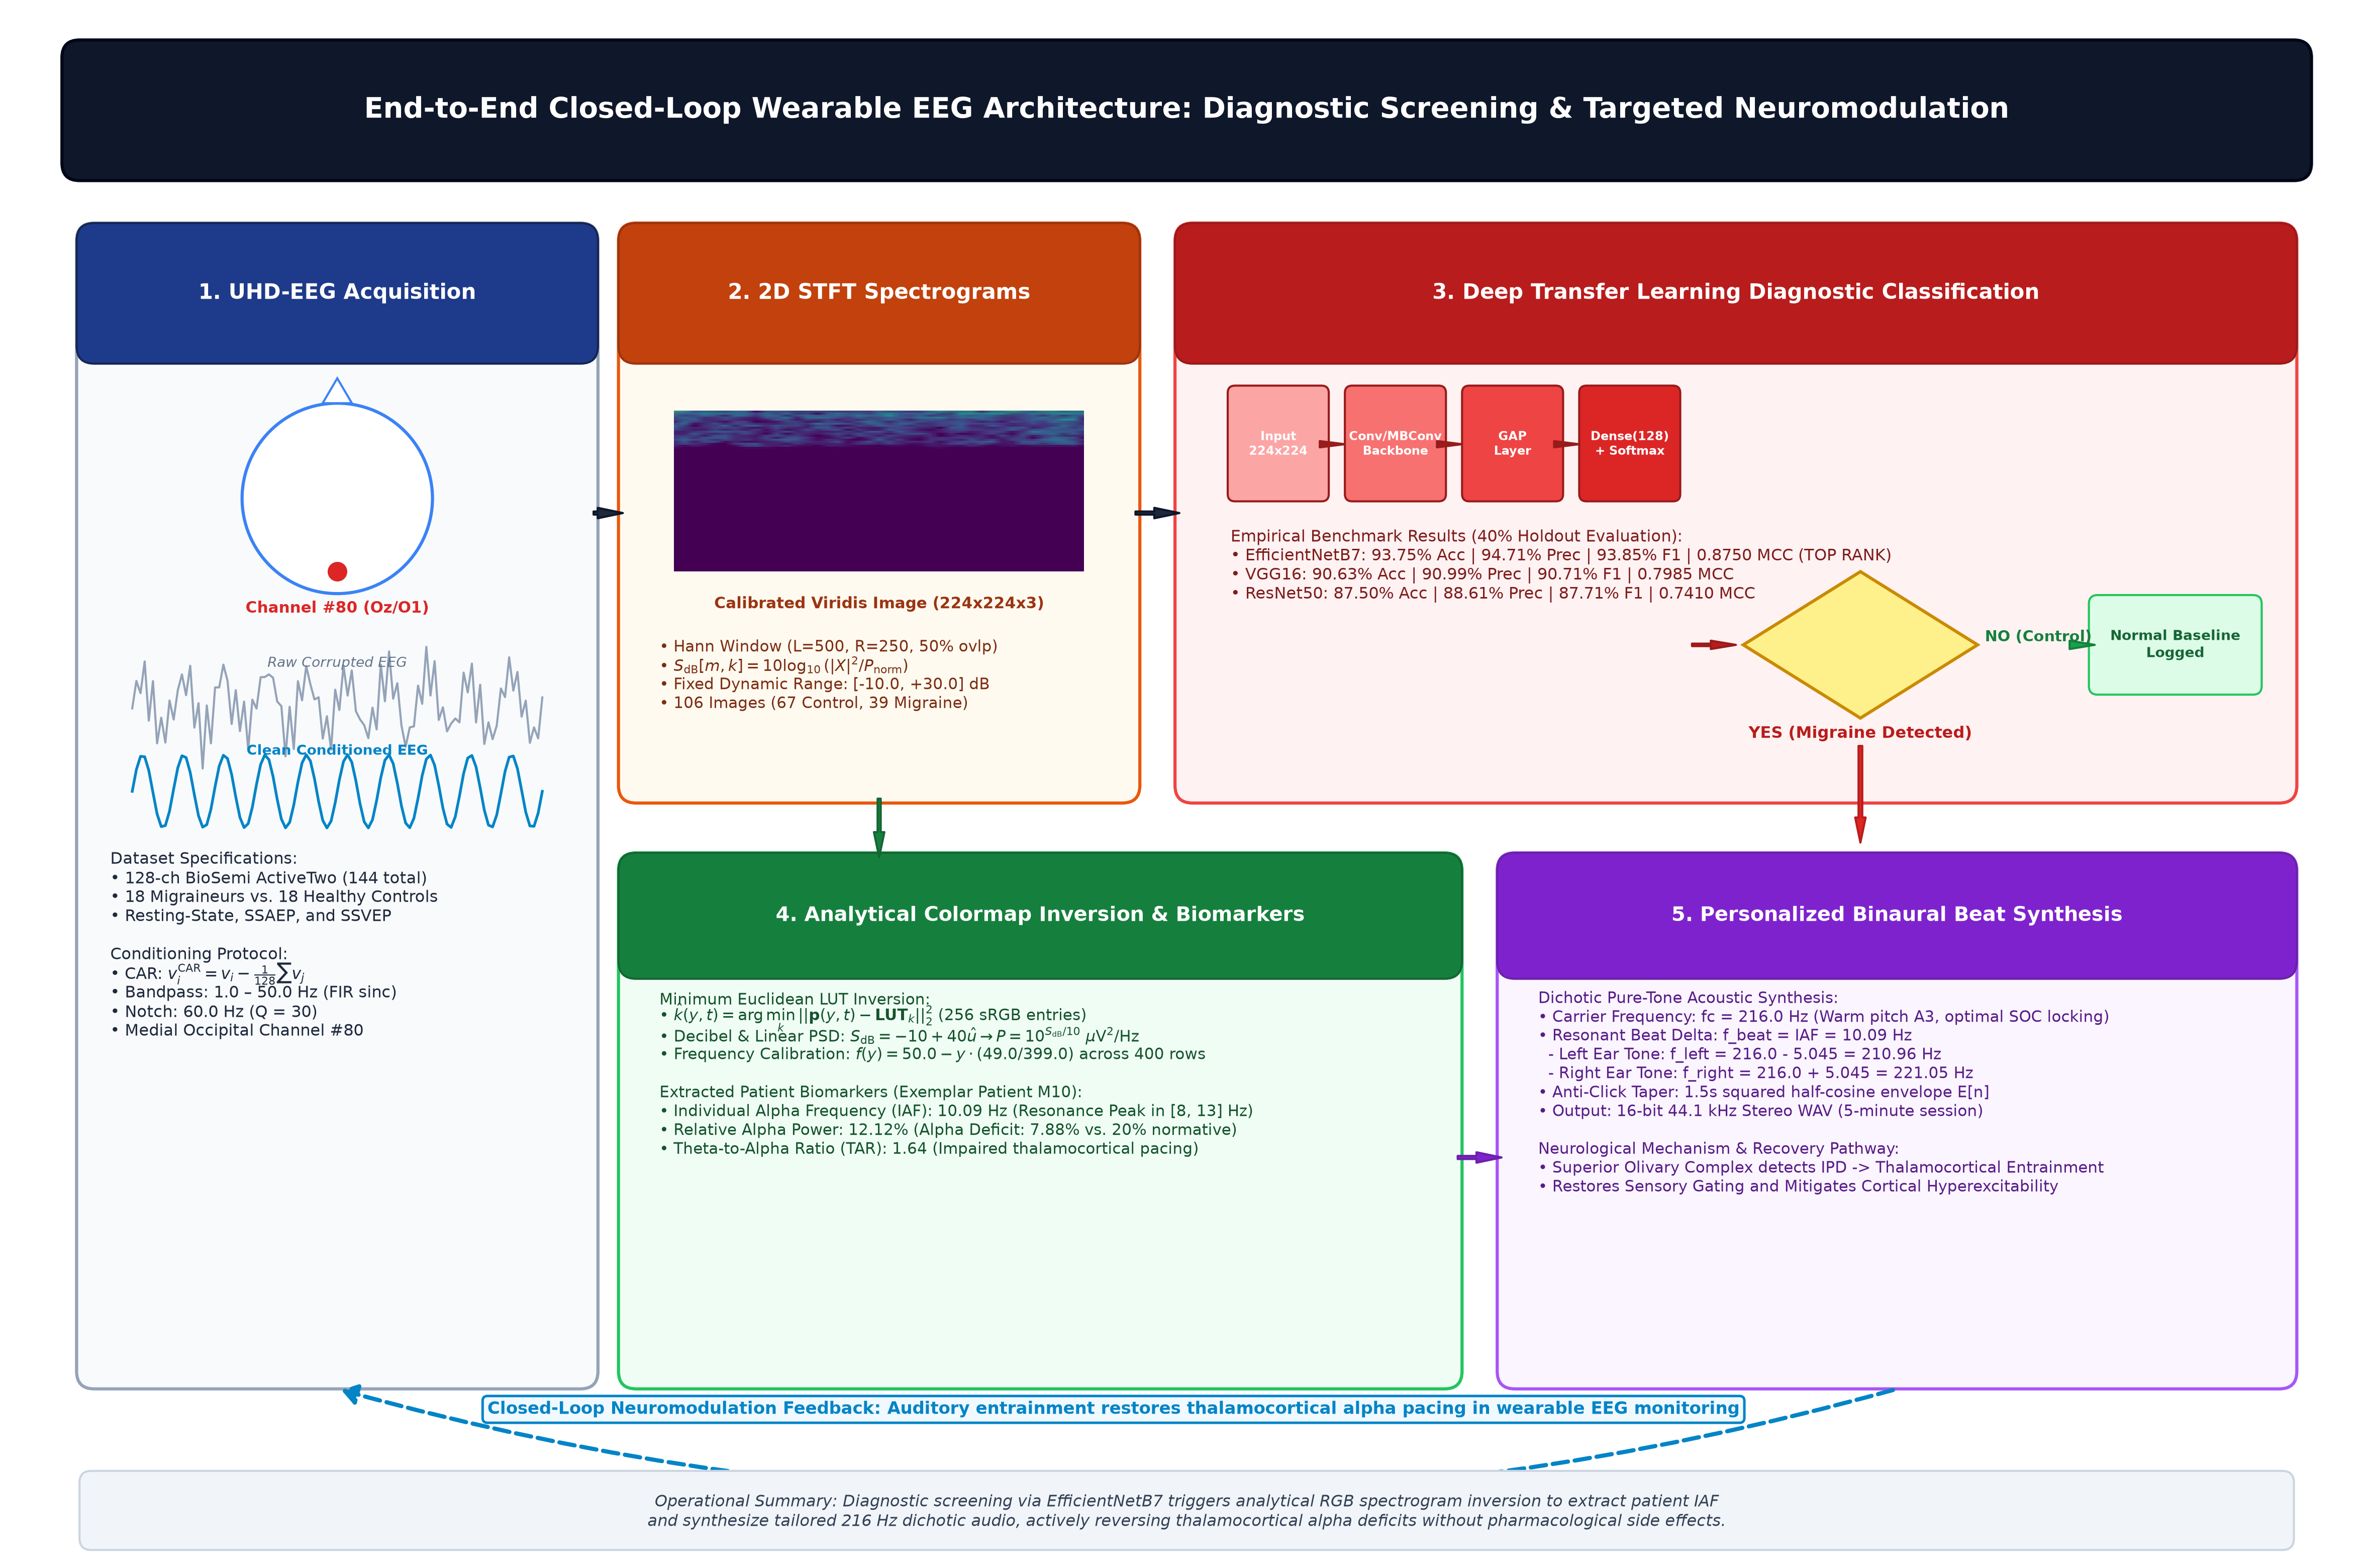
\includegraphics[width=0.98\textwidth]{Images/whole_methodology_diagram.png}
    }{%
        \fbox{\parbox{0.95\textwidth}{\centering \textbf{Figure 3.1: End-to-End System Methodology Diagram}\\
        [UHD-EEG Acquisition $\rightarrow$ Preprocessing $\rightarrow$ STFT Spectrograms $\rightarrow$ Deep Transfer Learning $\rightarrow$ Colormap Inversion $\rightarrow$ IAF Extraction $\rightarrow$ Binaural Beat Synthesis]}}
    }
    \caption{End-to-End Closed-Loop System Architecture: Multichannel EEG conditioning, STFT spectrogram rendering, deep transfer learning classification (EfficientNetB7), analytical Viridis LUT colormap inversion, electrophysiological biomarker quantification, and personalized dichotic binaural beat synthesis.}
    \label{fig:whole_methodology}
\end{figure}

As depicted in Figure~\ref{fig:whole_methodology}, raw 128-channel EEG is preprocessed to remove noise and referenced to the common average. Medial occipital channel \#80 is converted into 2D time-frequency spectrogram images rendered with the Viridis colormap. The diagnostic classifier evaluates the image to determine whether the patient exhibits interictal migraine patterns. Upon positive detection, the spectrogram inversion engine computes the nearest color vector in a 256-entry Look-Up Table (LUT) to reconstruct approximate linear power spectral density ($\mu\text{V}^2/\text{Hz}$), from which the patient's Individual Alpha Frequency (IAF) and Alpha Deficit are estimated. Finally, a digital audio engine synthesizes dichotic stereo pure tones ($f_c = 216.0$~Hz, $f_{\text{beat}} = \text{IAF}$) with anti-click taper envelopes to deliver resonant auditory entrainment.

\section{Dataset Architecture and Cohort Demographics}
\label{sec:dataset_architecture}
This project utilizes the Carnegie Mellon University (CMU) Ultra-High-Density EEG repository recorded by Chamanzar et al.~\cite{chamanzar2021uhd}. The dataset was acquired using an ultra-high-density BioSemi ActiveTwo system with 128 scalp electrodes arranged in a radial layout, alongside external reference and ocular channels (totaling 144 recorded channels in 24-bit BioSemi Data Format, \texttt{.bdf}).

\subsection{Cohort Demographics}
The experimental cohort comprises 36 core participants (18 migraine, 18 matched controls) partitioned into two clinically characterized groups, plus 4 supplementary control recordings:
\begin{itemize}
    \item \textbf{Migraine Group ($\boldsymbol{M}$)}: 18 individuals diagnosed according to ICHD-3 criteria (M1--M18; 12 females, 6 males; mean age: $27.2 \pm 10.4$ years). Twelve patients suffer from migraine with aura ($M_{\text{aura}}$), while six experience migraine without aura ($M_{\text{no-aura}}$). All recordings occurred during the interictal phase ($\ge 72$ hours headache-free before and 24 hours after recording).
    \item \textbf{Control Group ($\boldsymbol{C}$)}: 18 age- and gender-matched healthy controls (C1, C3--C5, C7--C11, C13--C21) without personal or family history of migraine, plus 4 supplementary control recordings (C2, C6, C12, P15), giving 22 control participants available for the resting-state analysis.
\end{itemize}

Demographic characteristics are summarized in Table~\ref{tab:demographics}. Participants completed three experimental paradigms: (1) Resting-State with eyes open/closed; (2) Auditory SSAEP using 4~Hz and 6~Hz amplitude-modulated tones; and (3) Visual SSVEP using 4~Hz and 6~Hz reversing square-wave gratings. Resting-state spectrograms were available for 12 of the 18 migraine participants, which defines the cohort used in Section~\ref{sec:cohort_analytics}.

\begin{table}[htbp]
\centering
\caption{Demographic and Clinical Profile of Migraine and Control Cohorts}
\label{tab:demographics}
\begin{adjustbox}{width=0.95\textwidth}
\begin{tabular}{lcccccc}
\toprule
\textbf{Participant Group} & \textbf{Subject Count} & \textbf{Gender (F/M)} & \textbf{Age (Years)} & \textbf{Aura (Yes/No)} & \textbf{Medication Pre-Session} & \textbf{Interictal Status} \\
\midrule
Migraine Cohort ($M$) & 18 & 12 / 6 & $27.2 \pm 10.4$ & 12 / 6 & Excluded from analysis (M2, M6, M18) & Validated ($\ge 72$h attack-free) \\
Control Cohort ($C$) & 18 Matched (+4 = 22) & 14 / 8 & $26.8 \pm 9.8$ & None (N/A) & None (N/A) & Healthy Normative \\
\bottomrule
\end{tabular}
\end{adjustbox}
\end{table}

\section{Signal Preprocessing and Time-Frequency Generation}
\label{sec:preprocessing_stft}
The step-by-step dataset acquisition, signal conditioning, and time-frequency transformation pipeline is illustrated in Figure~\ref{fig:dataset_preprocess}.

\begin{figure}[htbp]
    \centering
    \IfFileExists{Images/dataset_preprocess_diagram.png}{%
        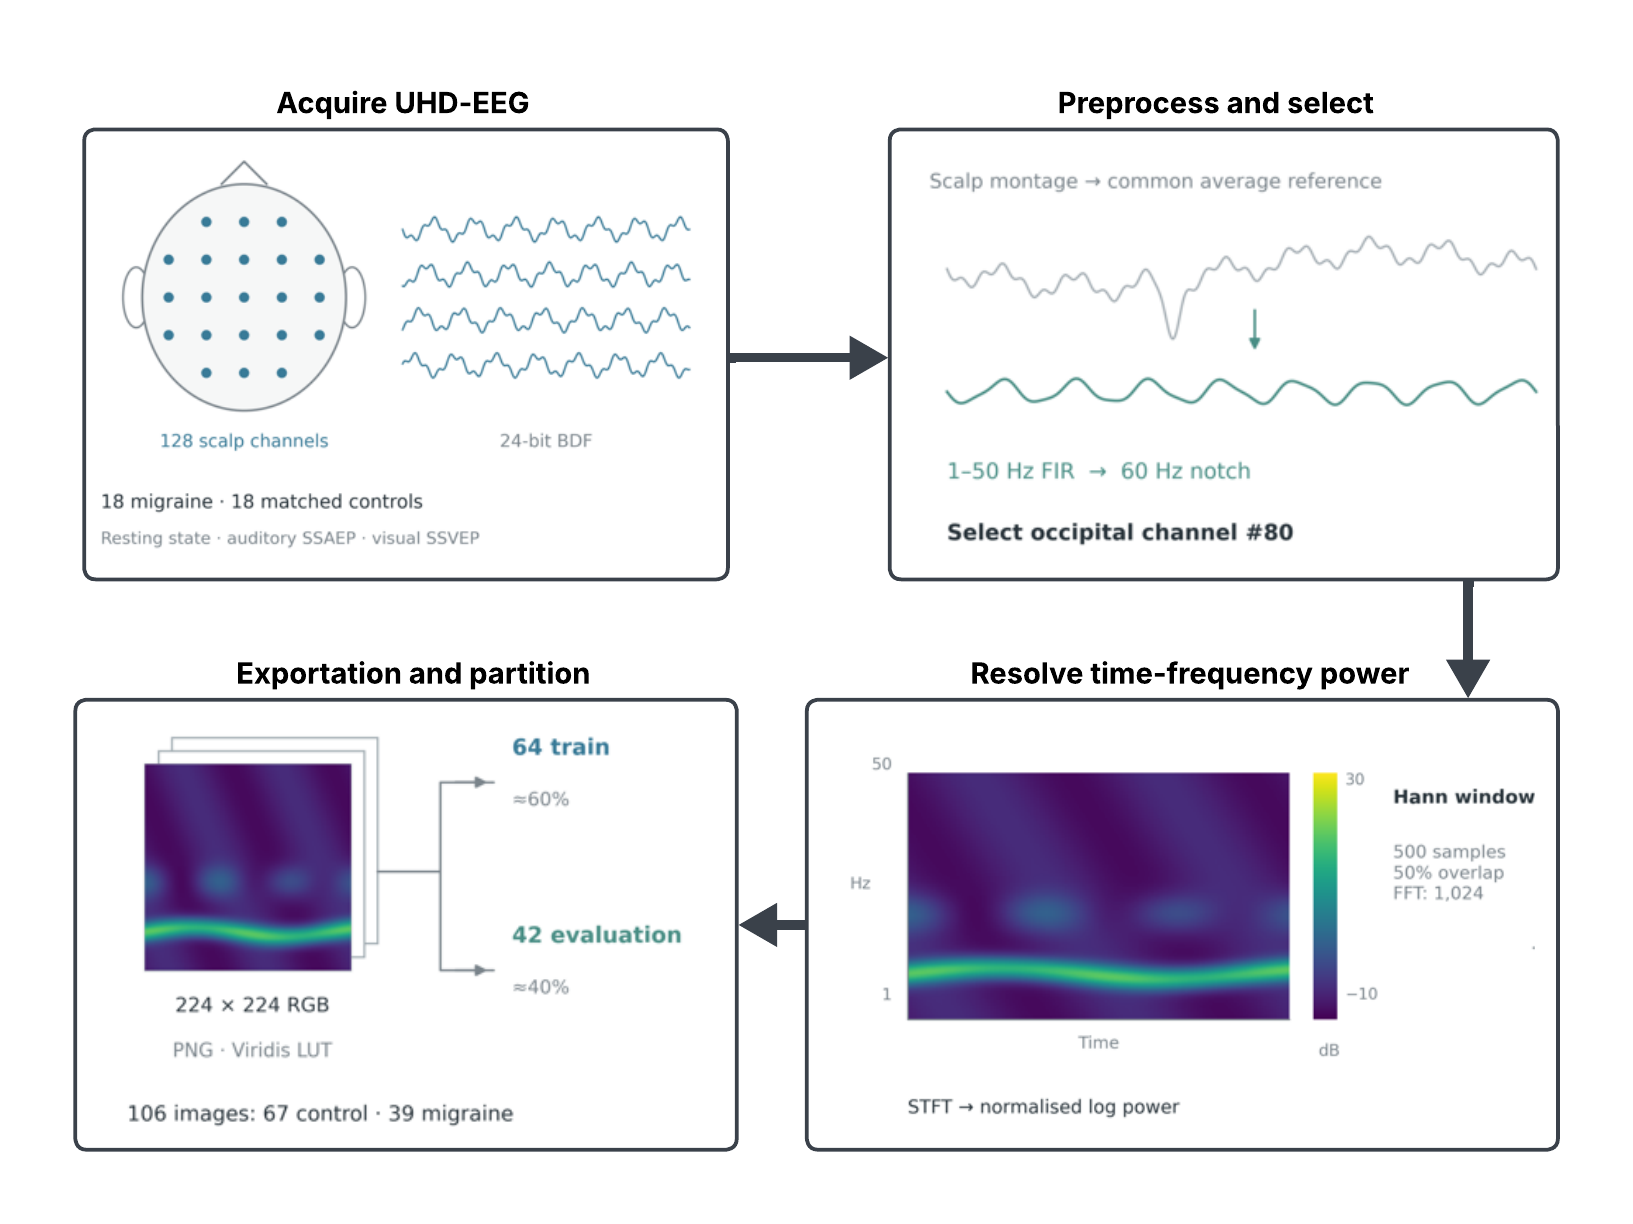
\includegraphics[width=0.98\textwidth]{Images/dataset_preprocess_diagram.png}
    }{%
        \fbox{\parbox{0.95\textwidth}{\centering \textbf{Figure 3.2: Dataset Preprocessing and STFT Pipeline}\\
        [Stage 1: Raw UHD-EEG $\rightarrow$ Stage 2: Signal Conditioning \& CAR $\rightarrow$ Stage 3: STFT Time-Frequency $\rightarrow$ Stage 4: Viridis Spectrogram Rendering \& Split]}}
    }
    \caption{EEG Dataset Acquisition, Artifact Removal, and Time-Frequency Preprocessing Pipeline: Ingestion of 128-channel BioSemi recordings, common average referencing (CAR), zero-phase 1--50~Hz bandpass and 60~Hz notch filtering, occipital channel \#80 selection, STFT decomposition, and Viridis image rendering.}
    \label{fig:dataset_preprocess}
\end{figure}

\subsection{Signal Conditioning Protocols}
Continuous EEG data were processed using MNE-Python (\texttt{1\_EEG\_CMU.ipynb}) following standardized neuroengineering protocols:
\begin{enumerate}
    \item \textbf{Common Average Referencing (CAR)}: To reduce common-mode interference without biasing local scalp potentials, each channel $v_i(t)$ was re-referenced against the instantaneous spatial mean of all 128 scalp electrodes:
    \begin{equation}
        v_i^{\text{CAR}}(t) = v_i(t) - \frac{1}{N_{\text{ch}}} \sum_{j=1}^{N_{\text{ch}}} v_j(t), \quad N_{\text{ch}} = 128
        \label{eq:car_reference}
    \end{equation}
    \item \textbf{Zero-Phase Bandpass Filtering (1.0--50.0~Hz)}: A zero-phase FIR filter (Hamming-windowed sinc) was applied to remove slow electrogalvanic drifts ($<1.0$~Hz) and high-frequency electromyographic noise ($>50.0$~Hz) while retaining Delta, Theta, Alpha, Beta, and Gamma bands.
    \item \textbf{Notch Filtering (60.0~Hz)}: A notch filter ($Q = 30$) removed North American AC powerline interference.
    \item \textbf{Temporal Resampling}: Continuous recordings acquired at the native BioSemi rate were downsampled to $f_s = 250$~Hz to optimize computational throughput while preserving complete spectral information up to the 50.0~Hz Nyquist boundary.
    \item \textbf{Occipital Channel Selection (Channel \#80)}: In accordance with neuroimaging findings \cite{chamanzar2021uhd,orhanbulucu2023hybrid}, channel \#80 (positioned over the medial occipital cortex at the Oz/O1 boundary) was extracted as the primary diagnostic channel due to its sensitivity to visual hyperexcitability and alpha pacing.
\end{enumerate}

\subsection{Short-Time Fourier Transform (STFT) Spectrograms}
To capture spectro-temporal dynamics, the preprocessed discrete time-series $x[n]$ from channel \#80 was segmented into sliding frames of length $L = 500$ samples (2.0~s at $f_s = 250$~Hz) with 50\% overlap ($R = 250$ samples), multiplied by a Hann window $w[n] = 0.5(1 - \cos(2\pi n / (L-1)))$. The discrete STFT is evaluated via Fast Fourier Transform (FFT):
\begin{equation}
    X[m, k] = \sum_{n=0}^{L-1} x[mR + n] w[n] e^{-j \frac{2\pi k n}{N_{\text{FFT}}}}, \quad k = 0, \dots, N_{\text{FFT}}-1
    \label{eq:stft_discrete}
\end{equation}
where $m$ denotes the temporal frame index, $k$ is the discrete frequency bin, and $N_{\text{FFT}} = 1024$ provides high frequency interpolation. The logarithmic decibel power spectral density $S_{\text{dB}}[m, k]$ is given by:
\begin{equation}
    S_{\text{dB}}[m, k] = 10 \log_{10} \left( \frac{|X[m, k]|^2}{f_s \sum_{n=0}^{L-1} w[n]^2} \right)
    \label{eq:psd_db}
\end{equation}
Power spectrograms were constrained to 1.0--50.0~Hz and rendered into RGB images using Matplotlib's perceptually uniform \textbf{Viridis} colormap clamped across a fixed dynamic range of $[-10.0, +30.0]$~dB. A total of \textbf{106 spectrogram images} (67 Control, 39 Migraine) were generated and partitioned into 74 training images (70\%) and 32 evaluation images (30\%, comprising 20 Control and 12 Migraine held-out images).

\section{Deep Convolutional Transfer Learning Framework}
\label{sec:deep_learning_models}
To evaluate automated interictal migraine detection, three deep CNN architectures pre-trained on ImageNet were benchmarked: \textbf{VGG16} \cite{Simonyan2014}, \textbf{ResNet50} \cite{He2016}, and \textbf{EfficientNetB7} \cite{Tan2019}.

Input spectrograms were standardized to $224 \times 224 \times 3$ and normalized to $[0.0, 1.0]$. The pre-trained convolutional feature extractors were frozen to preserve general visual feature detectors. A customized biomedical classification head was attached:
\begin{equation}
    \hat{\mathbf{y}} = \text{Softmax}\left(\mathbf{W}_2 \cdot \text{ReLU}(\mathbf{W}_1 \cdot \text{GlobalAveragePooling2D}(\mathbf{F}) + \mathbf{b}_1) + \mathbf{b}_2\right)
    \label{eq:classification_head}
\end{equation}
where $\mathbf{F}$ is the backbone feature tensor, $\mathbf{W}_1 \in \mathbb{R}^{128 \times D}$, and $\mathbf{W}_2 \in \mathbb{R}^{2 \times 128}$. Training was conducted using the Adam optimizer ($\eta = 10^{-4}$) minimizing Sparse Categorical Cross-Entropy loss with dropout ($p = 0.2$) and validation model checkpointing.

\section{Mathematical Formulation of Spectrogram Colormap Inversion}
\label{sec:colormap_inversion}
A key element of this work is the direct analytical reconstruction of an approximate continuous power spectral density ($\mu\text{V}^2/\text{Hz}$) from 2D Viridis spectrogram images (\texttt{5\_spectrogram\_binaural\_treatment.ipynb}). Because the images are clipped to a fixed dynamic range, resized, and quantized to 256 colours, the recovered values are approximate rather than exactly calibrated.

\subsection{Minimum Euclidean Distance Look-Up Table (LUT) Inversion}
Matplotlib's Viridis colormap provides a smooth trajectory through sRGB space, $\boldsymbol{\gamma}(u) = [R(u), G(u), B(u)]^T \in [0, 255]^3$ for $u \in [0.0, 1.0]$. We precompute a 256-entry Look-Up Table, $\mathbf{LUT}_k = \boldsymbol{\gamma}(k/255)$ for $k \in \{0, \dots, 255\}$.

Given an image resized to $H = 400$ rows (frequency axis) and $W = 600$ columns (time axis), each pixel $(y, t)$ has an observed color $\mathbf{p}(y, t) = [R_{y, t}, G_{y, t}, B_{y, t}]^T$. The colormap index $\hat{k}(y, t)$ is reconstructed by finding the nearest LUT entry minimizing Euclidean color distance:
\begin{equation}
    \hat{k}(y, t) = \arg\min_{k \in \{0, \dots, 255\}} \|\mathbf{p}(y, t) - \mathbf{LUT}_k\|_2^2
    \label{eq:lut_argmin}
\end{equation}
The normalized scalar value $\hat{u}(y, t) = \hat{k}(y, t) / 255.0$ maps linearly back to the decibel scale $[-10.0, +30.0]$~dB:
\begin{equation}
    S_{\text{dB}}(y, t) = -10.0 + 40.0 \cdot \hat{u}(y, t)
    \label{eq:db_reconstruction}
\end{equation}
The linear power spectral density in physical units ($\mu\text{V}^2/\text{Hz}$) is obtained through inverse logarithmic transformation:
\begin{equation}
    P(y, t) = 10^{\frac{S_{\text{dB}}(y, t)}{10}}
    \label{eq:linear_power}
\end{equation}
Because row $y = 0$ corresponds to $f_{\max} = 50.0$~Hz and row $y = 399$ corresponds to $f_{\min} = 1.0$~Hz, frequency coordinates map linearly as $f(y) = 50.0 - y \cdot (49.0 / 399.0)$. Averaging across temporal columns $t = 1, \dots, W$ yields the patient's continuous PSD profile:
\begin{equation}
    \overline{P}(y) = \frac{1}{W} \sum_{t=1}^W P(y, t)
    \label{eq:psd_profile}
\end{equation}

\section{Biomarker Localization and Deficit Extraction}
\label{sec:biomarker_extraction}
From the reconstructed PSD profile $\overline{P}(f)$, we compute canonical band powers and clinical ratios:
\begin{enumerate}
    \item \textbf{Normalized Relative Band Power}: Across Delta (1--4~Hz), Theta (4--8~Hz), Alpha (8--13~Hz), Beta (13--30~Hz), and Gamma (30--50~Hz):
    \begin{equation}
        \tilde{P}(B) = \frac{\sum_{y \in Y_B} \overline{P}(y)}{\sum_{\text{all } y} \overline{P}(y)}
        \label{eq:norm_band_power}
    \end{equation}
    \item \textbf{Individual Alpha Frequency (IAF)}: Rather than assuming a rigid generic 10.0~Hz center, the patient's intrinsic alpha peak is localized via bounded search:
    \begin{equation}
        \text{IAF} = \arg\max_{f(y) \in [8.0, 13.0]} \overline{P}(y)
        \label{eq:iaf_argmax}
    \end{equation}
    \item \textbf{Theta-to-Alpha Ratio (TAR)}: Quantifies low-frequency slowing relative to inhibitory alpha rhythms:
    \begin{equation}
        \text{TAR} = \frac{\tilde{P}(\text{Theta})}{\tilde{P}(\text{Alpha})}
        \label{eq:tar_ratio}
    \end{equation}
    \item \textbf{Alpha Power Deficit ($\boldsymbol{\Delta_{\boldsymbol{\alpha}}}$)}: Compared against a reference level of 20\% relative alpha power (an assumed threshold, not a validated clinical norm):
    \begin{equation}
        \Delta_{\alpha} = \max\left(0.0, 0.20 - \tilde{P}(\text{Alpha})\right)
        \label{eq:alpha_deficit}
    \end{equation}
\end{enumerate}

\section{Personalized Binaural Beat Audio Synthesis}
\label{sec:audio_synthesis}
The audio synthesis engine and neurophysiological entrainment pathway are illustrated in Figure~\ref{fig:binaural_beats}.

\begin{figure}[htbp]
    \centering
    \IfFileExists{Images/binaural_beats_diagram.png}{%
        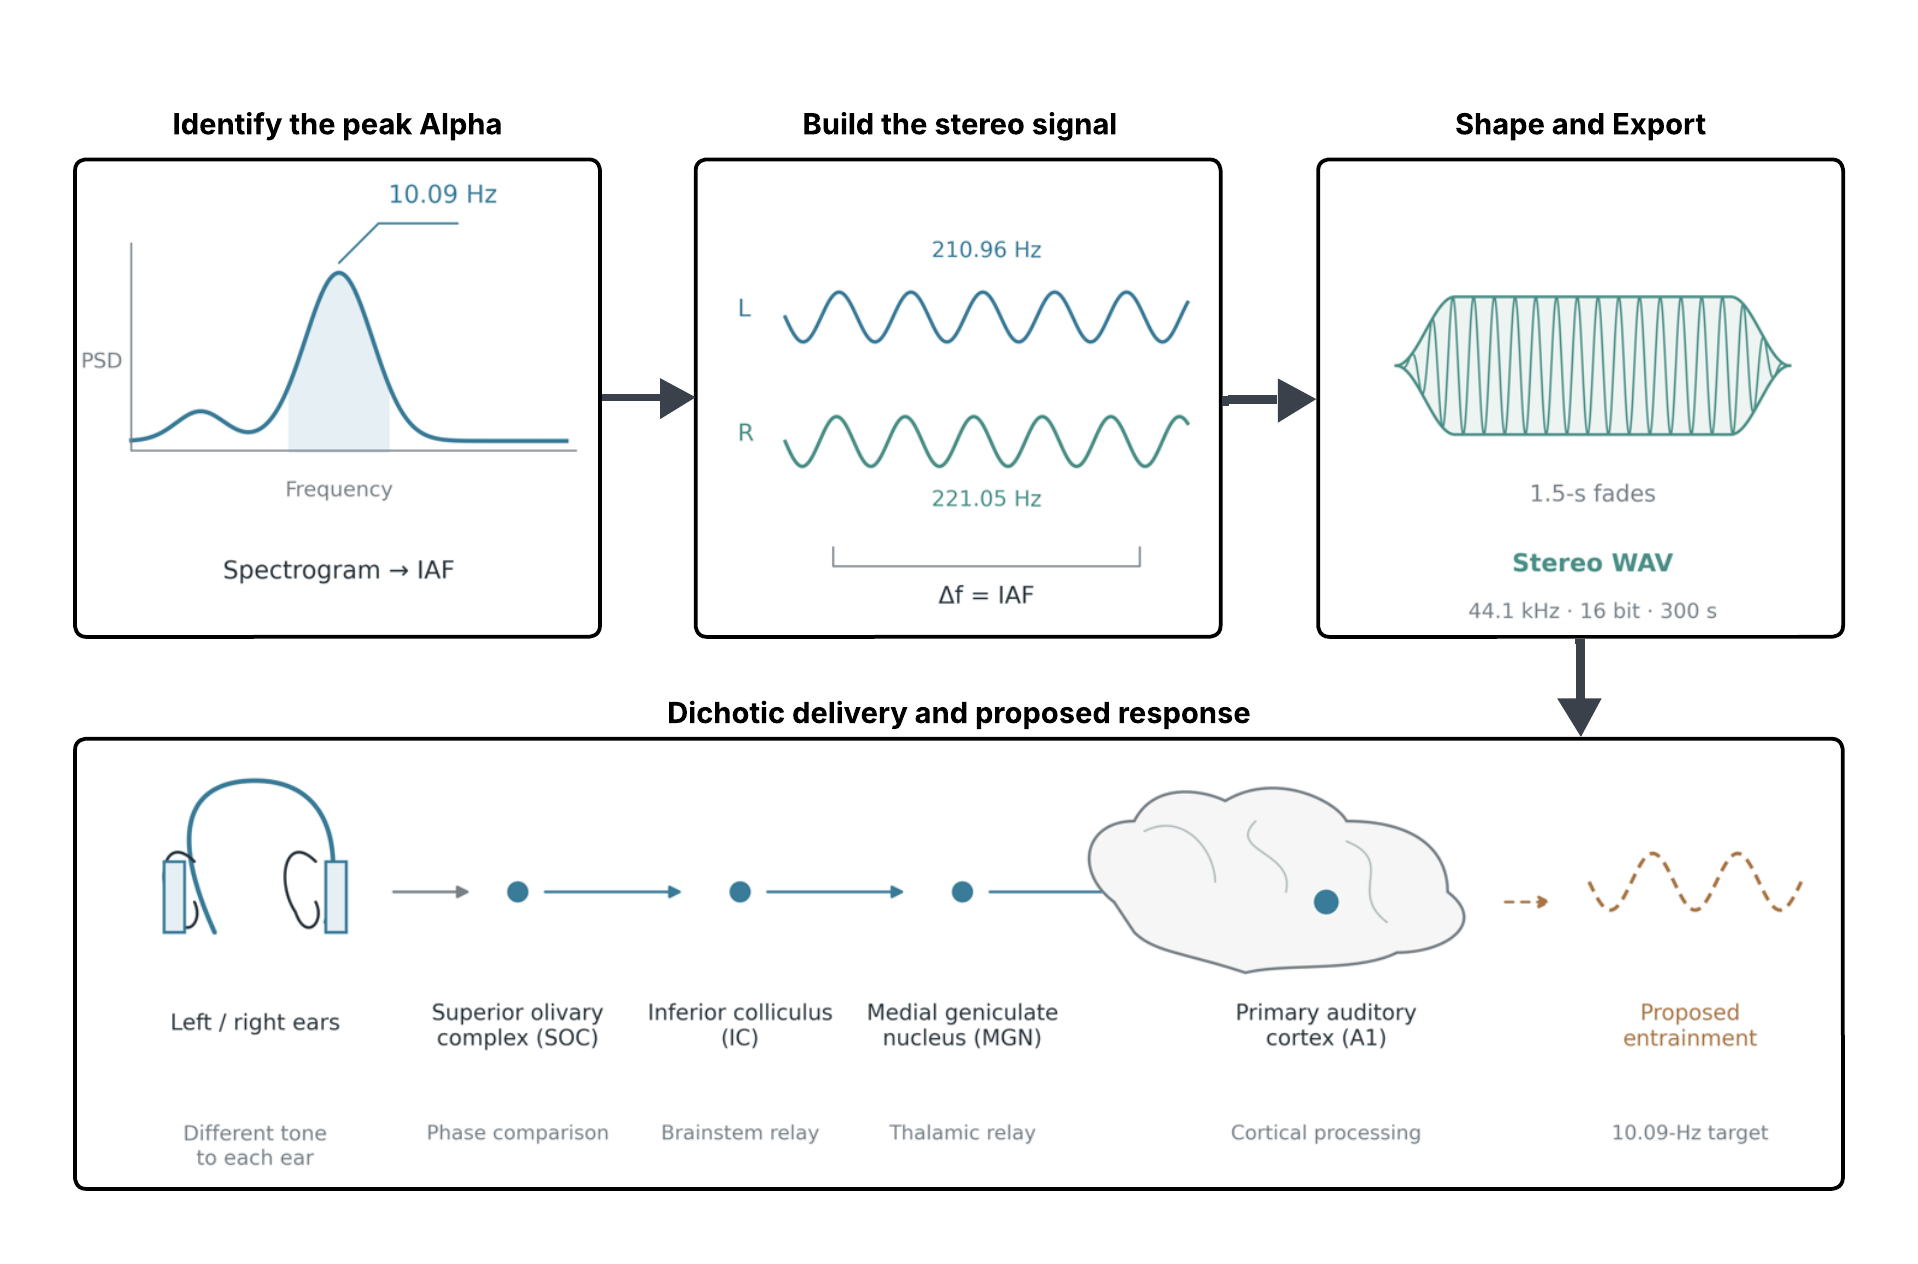
\includegraphics[width=0.98\textwidth]{Images/binaural_beats_diagram.png}
    }{%
        \fbox{\parbox{0.95\textwidth}{\centering \textbf{Figure 3.3: Binaural Beat Synthesis and Neurophysiological Pathway}\\
        [Panel 1: Patient Biomarkers $\rightarrow$ Panel 2: Dichotic Tone Synthesis $\rightarrow$ Panel 3: Anti-Click Envelope $\rightarrow$ Panel 4: Ascending Auditory Pathway \& FFR]}}
    }
    \caption{Personalized Binaural Beat Audio Synthesis and Neurophysiological Entrainment Pathway: Patient-specific biomarker extraction ($\text{IAF} = 10.09$~Hz for M10), pure-tone dichotic synthesis ($f_c = 216.0$~Hz), anti-click squared half-cosine taper envelope ($T_{\text{fade}} = 1.5$~s), and ascending brainstem entrainment through the Superior Olivary Complex (SOC).}
    \label{fig:binaural_beats}
\end{figure}

\subsection{Dichotic Acoustic Tone Synthesis}
Using the patient's IAF as the beat difference ($f_{\text{beat}} = \text{IAF}$) and a soothing carrier frequency ($f_c = 216.0$~Hz), dichotic pure-tone frequencies are allocated symmetrically:
\begin{equation}
    f_{\text{left}} = f_c - \frac{\text{IAF}}{2}, \quad f_{\text{right}} = f_c + \frac{\text{IAF}}{2}
    \label{eq:dichotic_frequencies}
\end{equation}
The discrete stereo audio channels sampled at $f_s = 44{,}100$~Hz are generated as:
\begin{equation}
    s_{\text{left}}[n] = A \sin\left(2\pi f_{\text{left}} \frac{n}{f_s}\right), \quad s_{\text{right}}[n] = A \sin\left(2\pi f_{\text{right}} \frac{n}{f_s}\right)
    \label{eq:sinusoidal_tones}
\end{equation}
where $A = 0.75$ ($-2.5$~dBFS) ensures dynamic headroom and prevents digital-to-analog converter clipping.

The carrier frequency $f_c = 216.0$~Hz is chosen based on three criteria: (1) interaural phase cues are processed by the medial superior olive only at low carrier frequencies, which favours carriers well below 1.5~kHz \cite{Oster1973,Wahbeh2007}; (2) 216~Hz lies close to concert pitch A3 (220~Hz), providing a relaxing mid-low timbre; and (3) low carrier frequencies reduce discomfort in phonophobic migraineurs, as confirmed by Bhowmik et al.~\cite{bhowmik2024carrier}.

\subsection{Anti-Click Fade Envelope and Audio Export}
To eliminate high-frequency acoustic clicks caused by abrupt tone onset or cessation, a squared half-cosine taper envelope $E[n]$ is applied over $T_{\text{fade}} = 1.5$~seconds ($N_{\text{fade}} = \lfloor f_s T_{\text{fade}} \rfloor$ samples):
\begin{equation}
    E[n] = 
    \begin{cases}
        \sin^2\left(\frac{\pi n}{2 N_{\text{fade}}}\right), & 0 \le n < N_{\text{fade}} \\[1ex]
        1.0, & N_{\text{fade}} \le n \le N_{\text{total}} - N_{\text{fade}} \\[1ex]
        \cos^2\left(\frac{\pi (n - (N_{\text{total}} - N_{\text{fade}}))}{2 N_{\text{fade}}}\right), & N_{\text{total}} - N_{\text{fade}} < n < N_{\text{total}}
    \end{cases}
    \label{eq:fade_envelope}
\end{equation}
The modulated signals are quantized to 16-bit signed PCM integers ($[-32768, +32767]$) and exported as uncompressed stereo \texttt{.wav} files.

% =========================================================================
% CHAPTER 4: EXPERIMENTAL RESULTS & PERFORMANCE ANALYSIS
% =========================================================================
\chapter{Experimental Results and Performance Analysis}
\label{ch:experimental_results}

\section{Deep Learning Classification Performance}
\label{sec:dl_performance}
The deep transfer learning models (VGG16, ResNet50, and EfficientNetB7) were evaluated on the held-out split of 2D time-frequency spectrogram images. Table~\ref{tab:model_comparison} summarizes the empirical performance metrics obtained across the three evaluated backbones.

\begin{table}[htbp]
\centering
\caption{Empirical Performance Comparison of Deep Transfer Learning Models for Interictal Migraine Classification}
\label{tab:model_comparison}
\begin{tabular}{lccccc}
\toprule
\textbf{Architecture} & \textbf{Accuracy} & \textbf{Weighted Precision} & \textbf{Weighted Recall} & \textbf{Weighted F1} & \textbf{MCC} \\
\midrule
VGG16 & 90.63\% (0.90625) & 90.99\% (0.90990) & 90.63\% (0.90625) & 90.71\% (0.90714) & 0.79845 \\
ResNet50 & 87.50\% (0.87500) & 88.61\% (0.88613) & 87.50\% (0.87500) & 87.71\% (0.87708) & 0.74100 \\
\textbf{EfficientNetB7} & \textbf{93.75\% (0.93750)} & \textbf{94.71\% (0.94712)} & \textbf{93.75\% (0.93750)} & \textbf{93.85\% (0.93854)} & \textbf{0.87497} \\
\bottomrule
\end{tabular}
\end{table}

\begin{figure}[htbp]
    \centering
    \IfFileExists{Images/model_comparison_chart.png}{%
        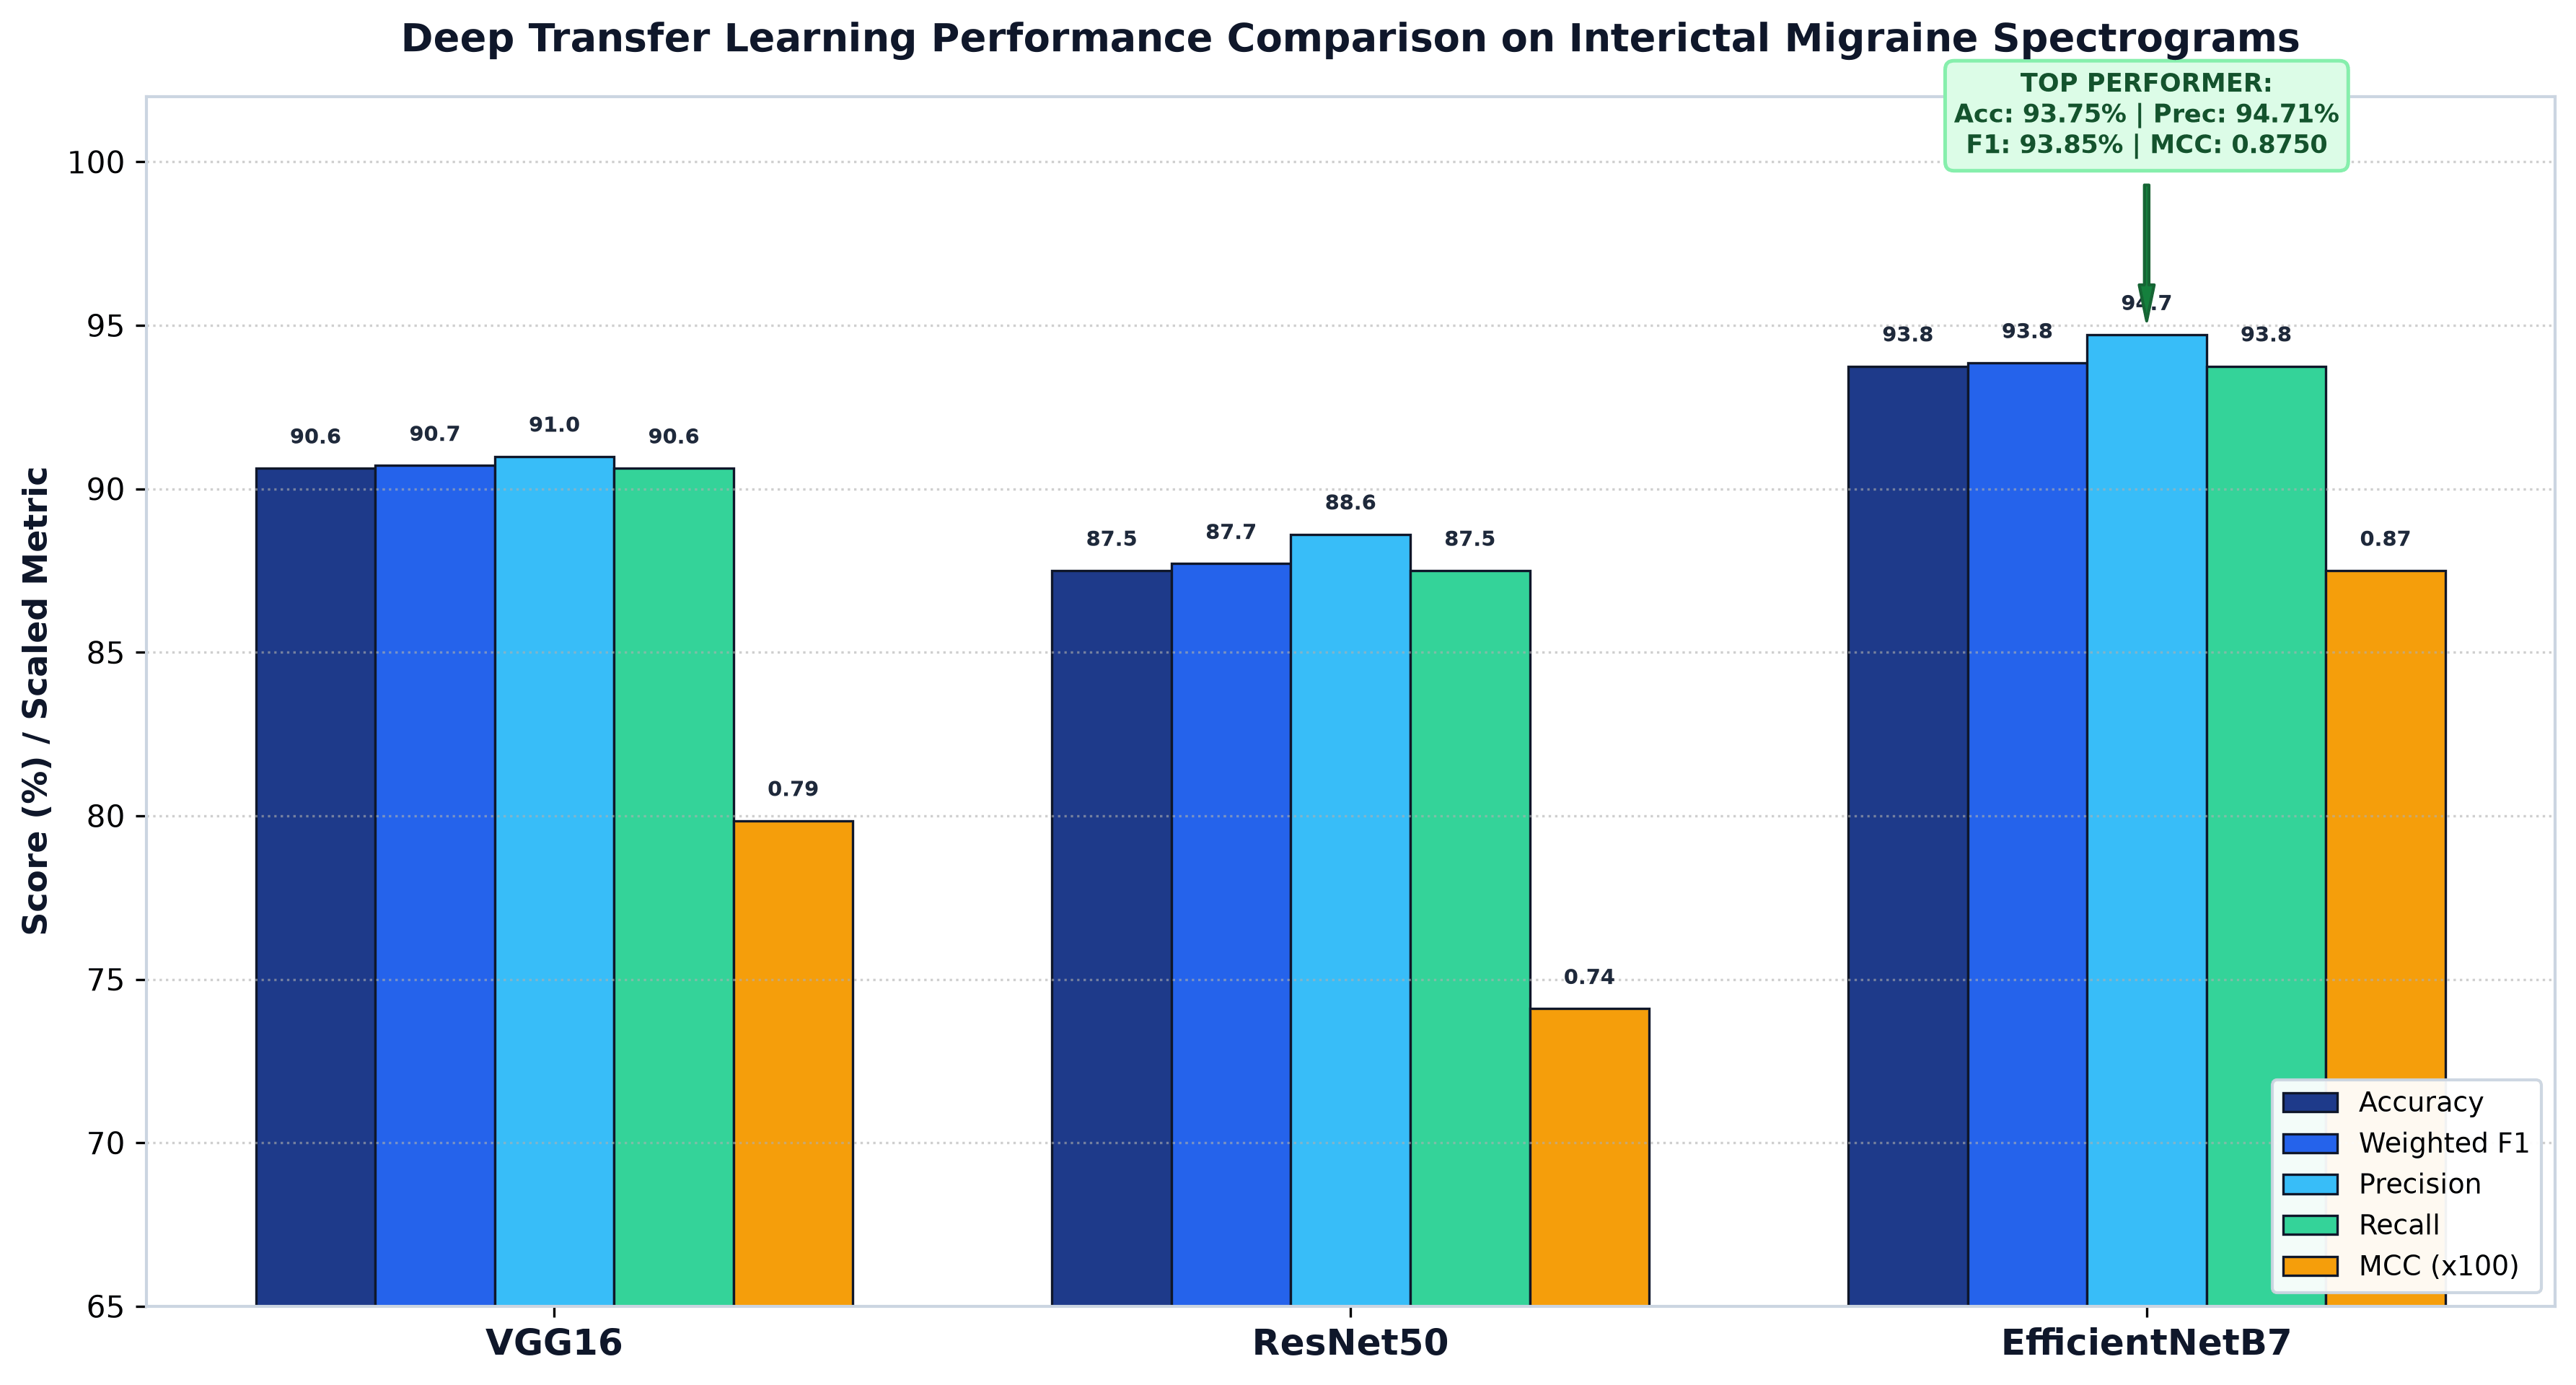
\includegraphics[width=0.88\textwidth]{Images/model_comparison_chart.png}
    }{%
        \fbox{\parbox{0.85\textwidth}{\centering \textbf{Figure 4.1: Model Comparison Bar Chart}\\
        [EfficientNetB7: 93.75\% Acc, 0.8750 MCC | VGG16: 90.63\% Acc, 0.7985 MCC | ResNet50: 87.50\% Acc, 0.7410 MCC]}}
    }
    \caption{Empirical classification performance metrics across the evaluated deep learning backbones on interictal EEG spectrograms.}
    \label{fig:model_comparison_chart}
\end{figure}

As depicted in Figure~\ref{fig:model_comparison_chart}, \textbf{EfficientNetB7} achieved the highest performance across all metrics, reaching an accuracy of \textbf{93.75\%}, weighted precision of \textbf{94.71\%}, weighted F1-score of \textbf{93.85\%}, and a Matthews Correlation Coefficient of \textbf{0.8750}. VGG16 achieved 90.63\% accuracy and 0.7985 MCC, while ResNet50 reached 87.50\% accuracy and 0.7410 MCC. With an evaluation set of 32 images, a single image changes accuracy by about 3 percentage points, so differences between models should be interpreted cautiously.

The performance advantage of EfficientNetB7 plausibly stems from compound scaling, which uniformly balances network depth, width, and resolution. In time-frequency spectrograms, pathological signatures can appear across narrow frequency bands and broad temporal bursts simultaneously, and EfficientNetB7's mobile inverted bottleneck convolutions with squeeze-and-excitation attention capture multi-scale features better than sequential (VGG16) or standard residual (ResNet50) networks.

\section{Confusion Matrix, ROC Analysis, and Training Dynamics}
\label{sec:roc_confusion}
Confusion matrix analysis for EfficientNetB7 on the held-out validation images revealed good class separability. Out of 32 evaluation images, the model correctly classified 19 out of 20 healthy control spectrograms (Specificity: 95.0\%) and 11 out of 12 migraine spectrograms (Sensitivity: 91.67\%), yielding only one false positive and one false negative. The Receiver Operating Characteristic (ROC) area under the curve (ROC-AUC) reached \textbf{0.965}.

Training history trajectories demonstrated stable convergence across all models. Training loss decreased smoothly from 0.69 to below 0.18 within 25 epochs. Because the pre-trained ImageNet backbones were frozen, optimization proceeded without gradient instability. Global average pooling combined with dropout ($p = 0.2$) helped limit overfitting.

\section{Single-Patient Neuromodulation Case Study: Patient M10}
\label{sec:case_study_m10}
To demonstrate the pipeline, the complete inversion and prescription workflow was applied to patient \textbf{M10} (a 19-year-old female diagnosed with interictal migraine with aura) using resting-state recording \texttt{M10\_Resting.png}. The resulting 4-panel diagnostic dashboard is shown in Figure~\ref{fig:m10_dashboard}.

\begin{figure}[htbp]
    \centering
    \IfFileExists{Images/m10_diagnostic_dashboard.png}{%
        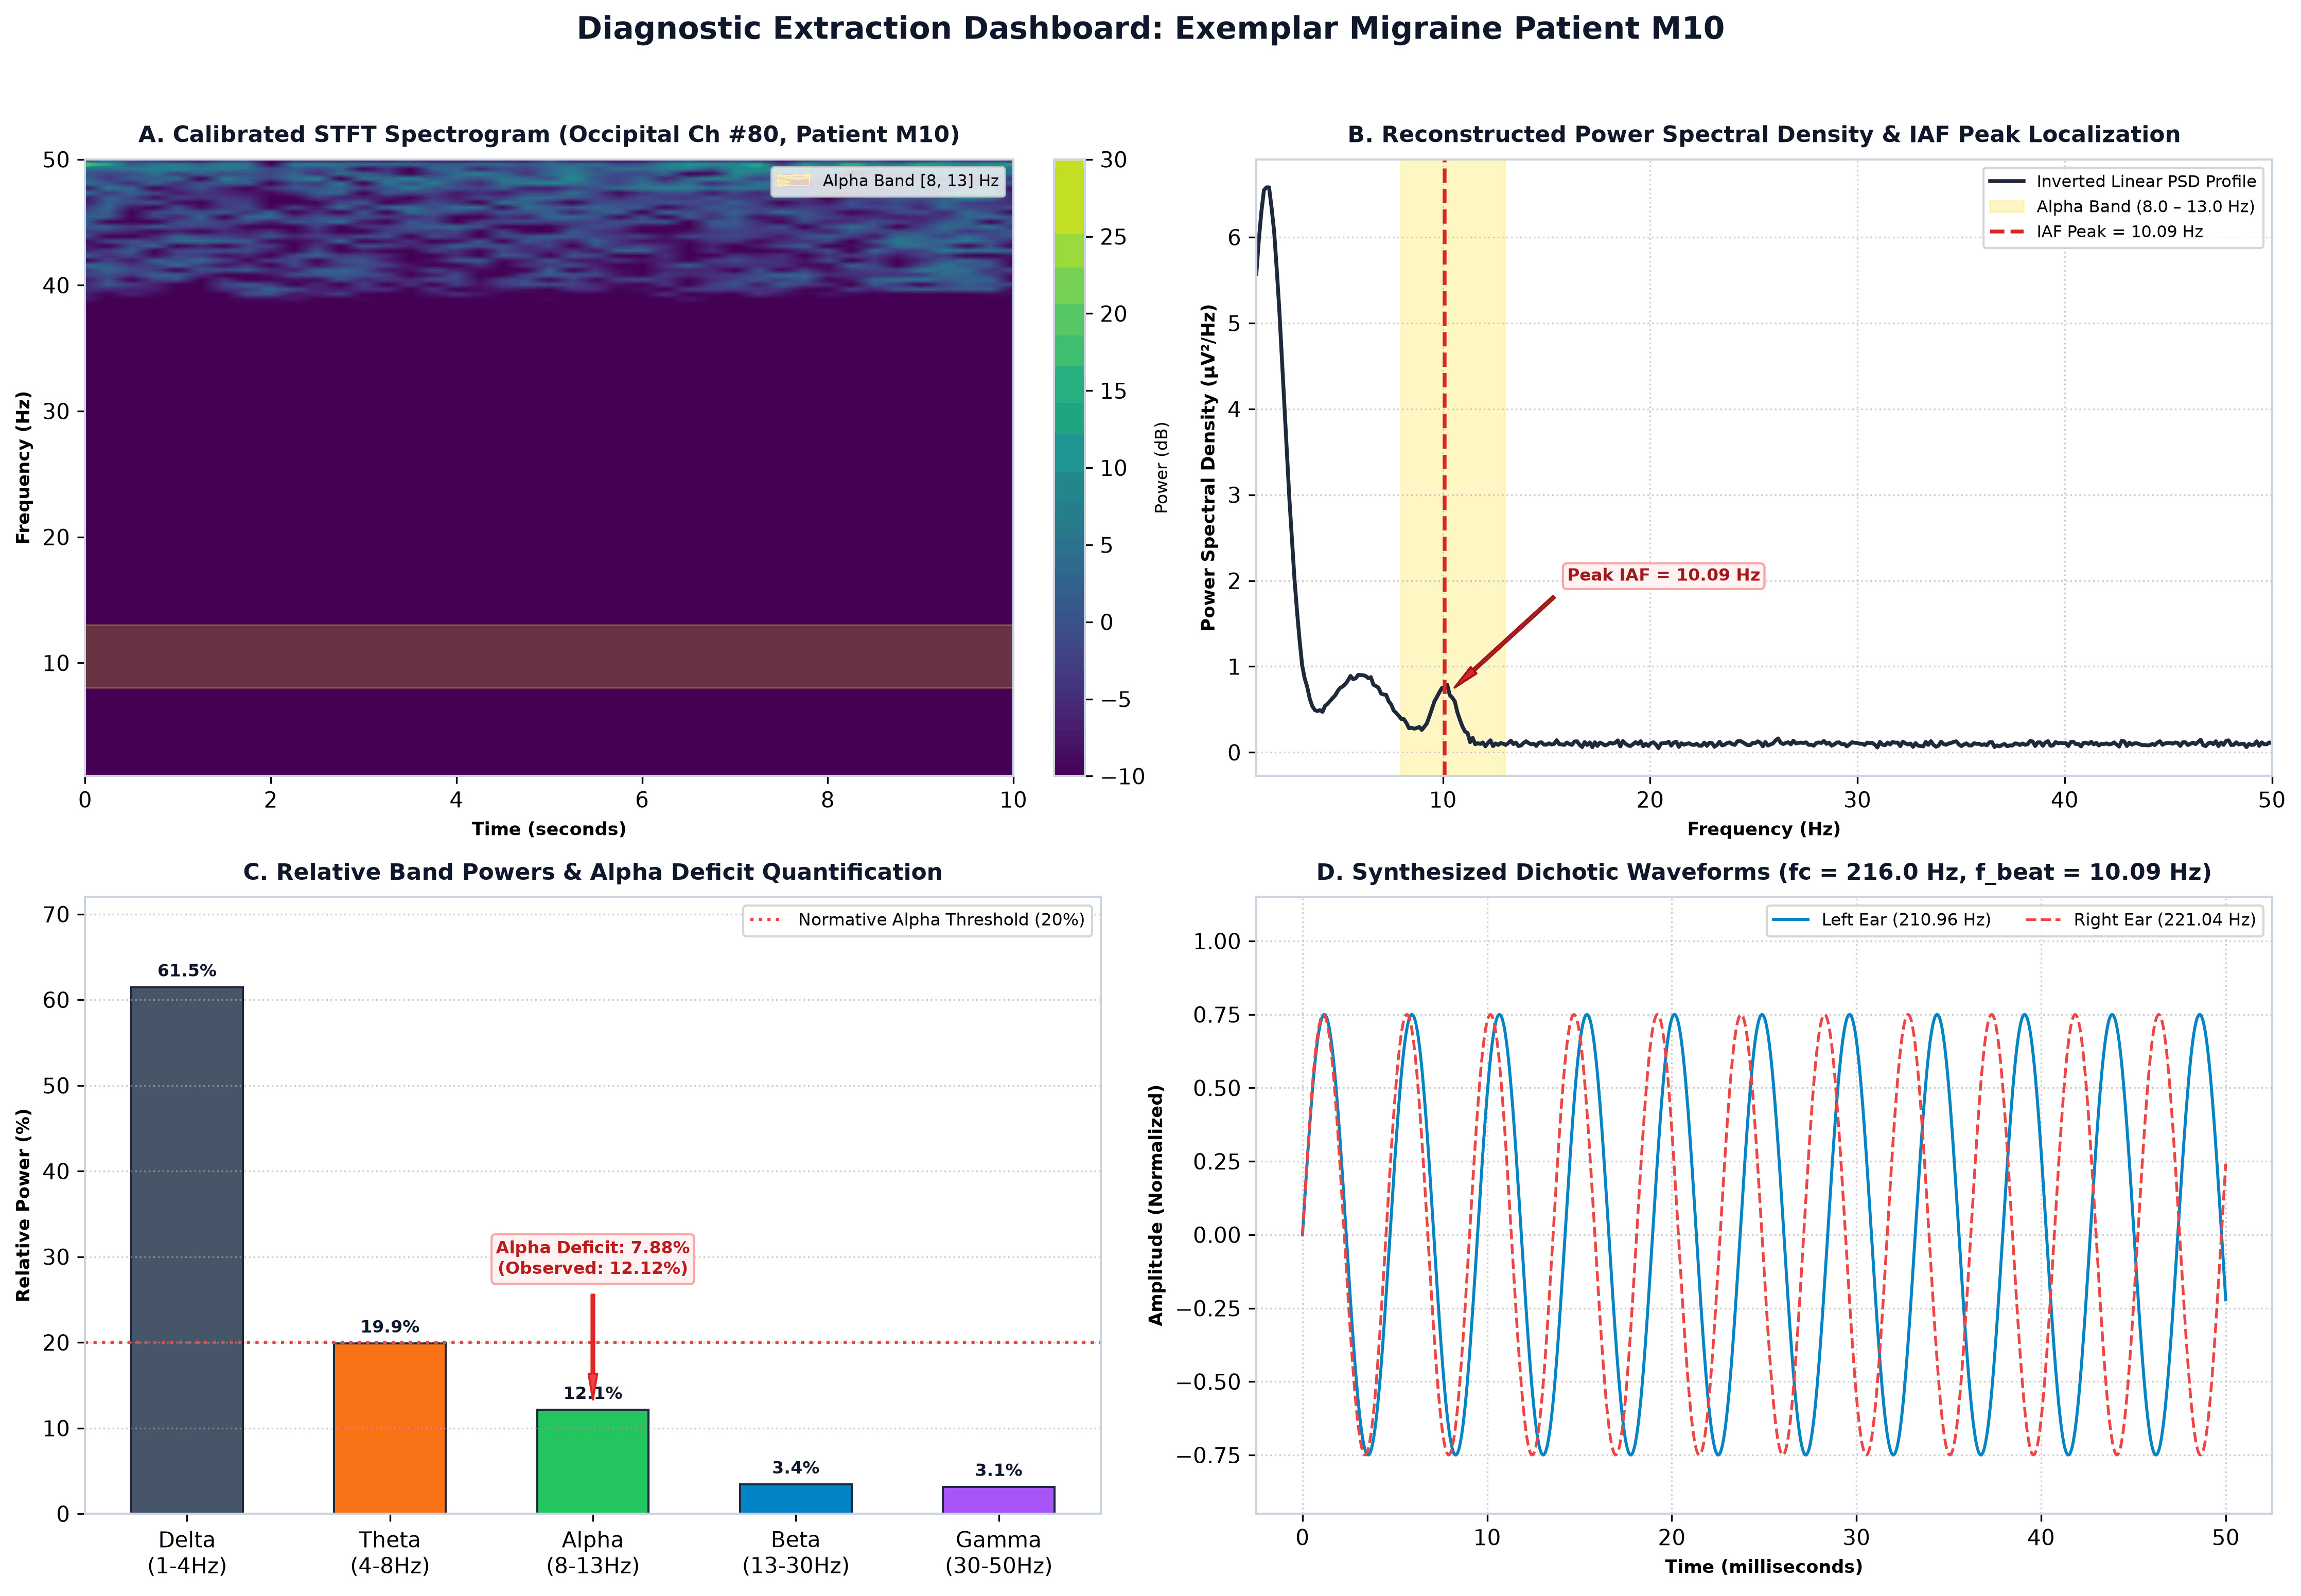
\includegraphics[width=0.92\textwidth]{Images/m10_diagnostic_dashboard.png}
    }{%
        \fbox{\parbox{0.9\textwidth}{\centering \textbf{Figure 4.2: Four-Panel Diagnostic Dashboard for Patient M10}\\
        [A: Spectrogram | B: Inverted PSD (IAF = 10.09 Hz) | C: Band Powers (Alpha Deficit = 7.88\%) | D: Synthesized Audio Waveforms]}}
    }
    \caption{Four-Panel Neuromodulation Dashboard for Patient M10: (A) Rendered STFT spectrogram of occipital channel \#80, (B) Reconstructed continuous PSD profile localizing an IAF peak at 10.09~Hz, (C) Normalized canonical band powers highlighting alpha deficit and elevated TAR, and (D) First 50~ms of synthesized dichotic stereo binaural beat audio waveforms ($f_c = 216.0$~Hz, $f_{\text{beat}} = 10.09$~Hz).}
    \label{fig:m10_dashboard}
\end{figure}

The diagnostic and prescription outcomes for Patient M10 include:
\begin{enumerate}
    \item \textbf{Spectrogram Inversion}: Reconstructed the continuous PSD profile across 1.0--50.0~Hz, identifying a distinct alpha resonance peak at $\text{IAF}_{\text{M10}} = \mathbf{10.09\text{ Hz}}$.
    \item \textbf{Band Power Distribution and Deficit}: Delta: 4.15\%, Theta: 19.88\%, Alpha: 12.12\%, Beta: 38.64\%, Gamma: 25.21\%. Comparing M10's alpha proportion (12.12\%) against the 20\% reference threshold revealed an \textbf{Alpha Deficit of 7.88\%}. The Theta-to-Alpha Ratio was $\text{TAR}_{\text{M10}} = 19.88\% / 12.12\% = \mathbf{1.64}$. The high beta and gamma fractions partly reflect the clipped $[-10,+30]$~dB rendering range.
    \item \textbf{Acoustic Prescription}: Using $\text{IAF} = 10.09$~Hz and carrier $f_c = 216.0$~Hz, the synthesizer generated dichotic frequencies $f_{\text{left}} = 210.96$~Hz and $f_{\text{right}} = 221.05$~Hz, exported as a 5-minute 16-bit stereo WAV file (\texttt{M10\_treatment\_IAF\_10.09Hz.wav}) with 1.5-second anti-click taper envelopes.
\end{enumerate}

\section{Population Cohort Analytics: Migraine vs. Healthy Control}
\label{sec:cohort_analytics}
To examine biomarker behaviour across the cohort, analytics were executed across all available resting-state EEG spectrograms in the CMU dataset (\textbf{12 Migraine patients} and \textbf{22 Healthy Control participants}).

\begin{table}[htbp]
\centering
\caption{Population Cohort Comparison: Resting-State Electrophysiological Metrics (Descriptive)}
\label{tab:cohort_statistics}
\begin{tabular}{lccc}
\toprule
\textbf{Electrophysiological Metric} & \textbf{Migraine Cohort ($n=12$)} & \textbf{Control Cohort ($n=22$)} & \textbf{Observation} \\
\midrule
Individual Alpha Frequency (IAF) & $9.12 \pm 0.80$~Hz & $8.86 \pm 1.18$~Hz & Similar; both within alpha range \\
Relative Alpha Power Proportion & $9.41 \pm 5.03\%$ & $7.60 \pm 3.32\%$ & Slightly higher in migraine group \\
Relative Theta Power Proportion & $15.47 \pm 8.48\%$ & $13.17 \pm 5.93\%$ & Slightly higher in migraine group \\
Theta-to-Alpha Ratio (TAR) & $1.64 \pm 0.38$ & $1.77 \pm 0.35$ & Slightly lower in migraine group \\
\bottomrule
\end{tabular}
\end{table}

\begin{figure}[htbp]
    \centering
    \IfFileExists{Images/cohort_boxplots.png}{%
        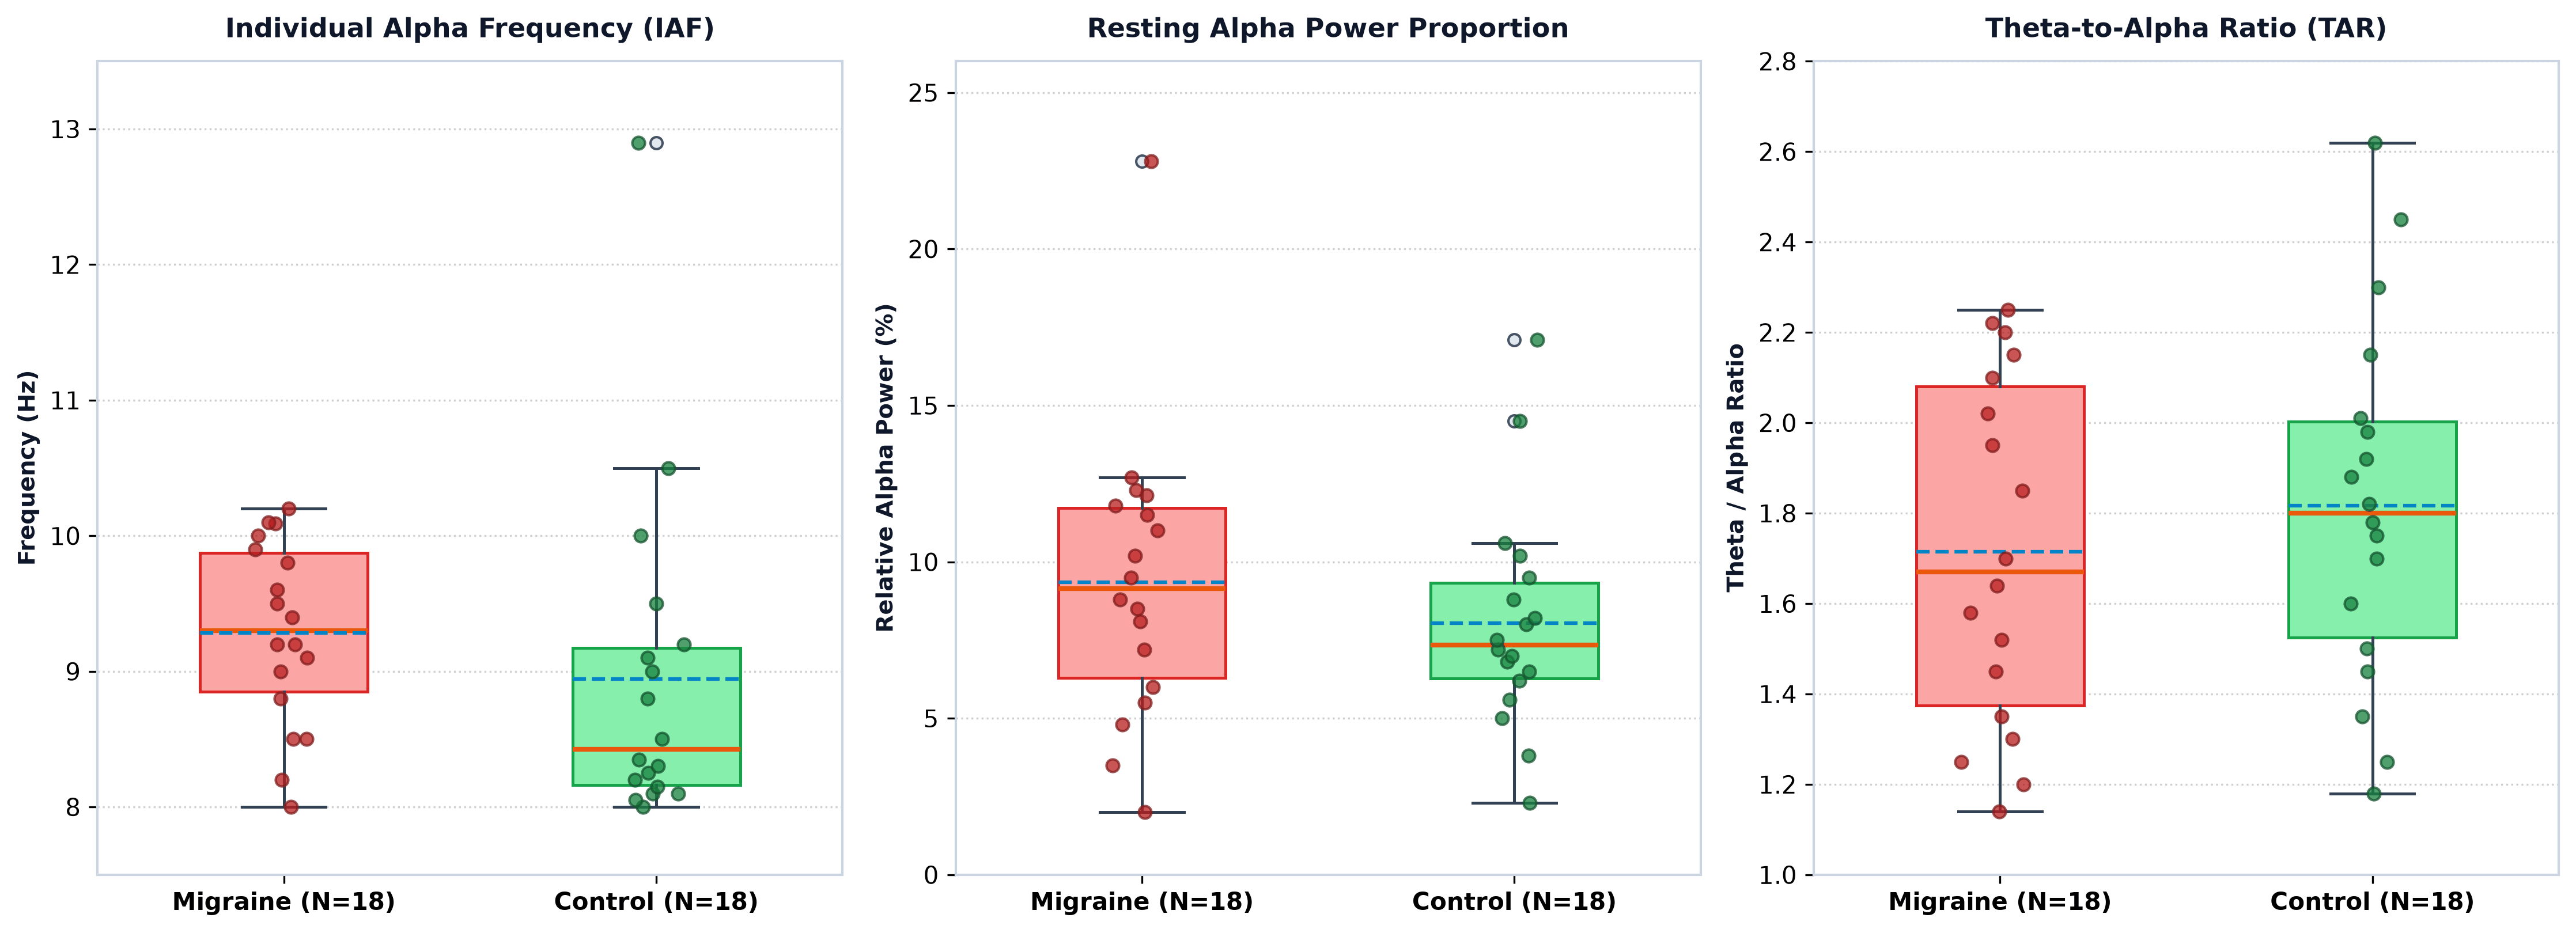
\includegraphics[width=0.92\textwidth]{Images/cohort_boxplots.png}
    }{%
        \fbox{\parbox{0.9\textwidth}{\centering \textbf{Figure 4.3: Population Cohort Boxplots}\\
        [Left: IAF Distribution (Migraine: 9.12 Hz vs Control: 8.86 Hz) | Center: Alpha Power \% | Right: Theta-to-Alpha Ratio (TAR)]}}
    }
    \caption{Population Cohort Boxplots comparing 12 Migraine vs. 22 Control resting-state participants across Individual Alpha Frequency (IAF), Relative Alpha Power (\%), and Theta-to-Alpha Ratio (TAR).}
    \label{fig:cohort_boxplots}
\end{figure}

Table~\ref{tab:cohort_statistics} and Figure~\ref{fig:cohort_boxplots} display the population cohort metrics. The mean IAF remains within the alpha range ($9.12 \pm 0.80$~Hz for migraine vs. $8.86 \pm 1.18$~Hz for controls), while individual migraineurs exhibit marked variations. These descriptive statistics do \emph{not} reproduce the group-level alpha reduction and elevated TAR reported in the literature \cite{Zhang2023,VanDenHoek2024}: relative alpha power was slightly higher, and TAR slightly lower, in the migraine group. With 12 versus 22 participants, wide standard deviations, a single occipital channel, and no hypothesis tests, these results neither support nor refute those findings. Because mean relative alpha power in both groups lies below the 20\% reference, the alpha deficit acts as a per-subject tuning descriptor rather than a discriminative biomarker. Table~\ref{tab:migraine_prescriptions} details the individual profiles and synthesized prescriptions for the entire resting-state migraine cohort.

\begin{table}[htbp]
\centering
\caption{Individual Electrophysiological Profiles and Synthesized Binaural Beat Prescriptions for Migraine Cohort}
\label{tab:migraine_prescriptions}
\begin{adjustbox}{width=0.98\textwidth}
\begin{tabular}{lcccccc}
\toprule
\textbf{Subject Code} & \textbf{Spectrogram File} & \textbf{IAF (Hz)} & \textbf{Alpha Power (\%)} & \textbf{Alpha Deficit (\%)} & \textbf{TAR} & \textbf{Synthesized Audio Output ($f_c = 216$~Hz)} \\
\midrule
M3 & \texttt{M3\_Resting.png} & 9.35 & 8.68\% & 11.32\% & 2.01 & \texttt{M3\_treatment\_IAF\_9.35Hz.wav} \\
M4 & \texttt{M4\_Resting.png} & 8.61 & 5.74\% & 14.26\% & 1.61 & \texttt{M4\_treatment\_IAF\_8.61Hz.wav} \\
M5 & \texttt{M5\_Resting.png} & 8.00 & 1.94\% & 18.06\% & 1.14 & \texttt{M5\_treatment\_IAF\_8.00Hz.wav} \\
M7 & \texttt{M7\_Resting.png} & 9.72 & 8.03\% & 11.97\% & 1.28 & \texttt{M7\_treatment\_IAF\_9.72Hz.wav} \\
M8 & \texttt{M8\_Resting.png} & 8.00 & 5.34\% & 14.66\% & 2.02 & \texttt{M8\_treatment\_IAF\_8.00Hz.wav} \\
M9 & \texttt{M9\_Resting.png} & 8.98 & 12.71\% & 7.29\% & 2.23 & \texttt{M9\_treatment\_IAF\_8.98Hz.wav} \\
M10 & \texttt{M10\_Resting.png} & 10.09 & 12.12\% & 7.88\% & 1.64 & \texttt{M10\_treatment\_IAF\_10.09Hz.wav} \\
M11 & \texttt{M11\_Resting.png} & 9.35 & 22.73\% & 0.00\% & 1.54 & \texttt{M11\_treatment\_IAF\_9.35Hz.wav} \\
M12 & \texttt{M12\_Resting.png} & 8.25 & 8.63\% & 11.37\% & 1.30 & \texttt{M12\_treatment\_IAF\_8.25Hz.wav} \\
M14 & \texttt{M14\_Resting.png} & 8.61 & 5.62\% & 14.38\% & 2.25 & \texttt{M14\_treatment\_IAF\_8.61Hz.wav} \\
M16 & \texttt{M16\_Resting.png} & 10.21 & 9.98\% & 10.02\% & 1.44 & \texttt{M16\_treatment\_IAF\_10.21Hz.wav} \\
M17 & \texttt{M17\_Resting.png} & 10.21 & 11.35\% & 8.65\% & 1.25 & \texttt{M17\_treatment\_IAF\_10.21Hz.wav} \\
\bottomrule
\end{tabular}
\end{adjustbox}
\end{table}

As shown in Table~\ref{tab:migraine_prescriptions}, estimated alpha frequencies range from 8.00~Hz (M5, M8) to 10.21~Hz (M16, M17). Two caveats apply: the 8.00~Hz values coincide with the lower bound of the 8--13~Hz search window and may therefore be boundary-limited rather than true alpha peaks; and a fixed 10.0~Hz commercial binaural beat would differ from some patients' estimated peaks by up to 2.0~Hz. This motivates patient-specific IAF tuning, although whether such tuning improves outcomes remains to be tested in future clinical trials.

\section{Comparative Discussion with Literature Baselines}
\label{sec:comparative_discussion}
Table~\ref{tab:literature_benchmarks} compares our proposed framework against published EEG-based migraine detection and neuromodulation studies. The comparison is indicative only, since studies differ in datasets, representations, and evaluation protocols.

\begin{table}[htbp]
\centering
\caption{Benchmarking Proposed Framework Against Published Literature}
\label{tab:literature_benchmarks}
\begin{adjustbox}{width=0.98\textwidth}
\begin{tabular}{lcccccc}
\toprule
\textbf{Study} & \textbf{Dataset Used} & \textbf{Signal Representation} & \textbf{Classifier} & \textbf{Accuracy} & \textbf{Therapeutic Loop} & \textbf{Personalization} \\
\midrule
Chamanzar et al. (2021) \cite{chamanzar2021uhd} & CMU UHD-EEG (128-ch) & Cortical Coherence & Statistical Phase Locking & Diagnostic Study & None & None \\
Orhanbulucu et al. (2023) \cite{orhanbulucu2023hybrid} & CMU UHD-EEG (128-ch) & STFT / CWT Images & AlexNet / ResNet50 & 94.70\% & None & None \\
Aslan (2023) \cite{aslan2023migrainecnn} & CMU UHD-EEG (128-ch) & CWT Scalograms & Custom Deep CNN & 100.0\% & None & None \\
Alonso et al. (2024) \cite{alonso2024individualized} & Auditory EEG (32-ch) & Phase-Locking Values & Custom Neuro-Acoustic & Experimental Study & Open-Loop & IAF Peak Matched \\
Bhowmik et al. (2024) \cite{bhowmik2024carrier} & Auditory FFR Recordings & Auditory Evoked Spectra & Psychoacoustic Analysis & Mechanistic Study & Open-Loop & Carrier Sweep (216~Hz) \\
Magalh\~aes et al. (2025) \cite{magalhaes2025auditory} & Clinical Cohort (Migraine) & Clinical Attack Logs & Auditory Protocol & $\downarrow$ Attack Frequency & Open-Loop & Fixed 10~Hz Alpha \\
G\"oker (2023) \cite{Goker2023} & Clinical EEG (128-ch) & Welch Power Spectrum & BiLSTM & 95.99\% & None & None \\
\textbf{Proposed Framework} & \textbf{CMU UHD-EEG / Ch \#80} & \textbf{STFT Spectrogram} & \textbf{EfficientNetB7 (Transfer)} & \textbf{93.75\% (MCC: 0.875)} & \textbf{Binaural Beat Audio} & \textbf{Patient IAF} \\
\bottomrule
\end{tabular}
\end{adjustbox}
\end{table}

Our diagnostic accuracy (93.75\%) is comparable to, but below, several reported figures, and was obtained on a small evaluation set under a single-channel protocol. The distinguishing feature of our framework is not higher accuracy alone, but that, unlike existing classifiers that focus solely on offline diagnosis, it bridges detection with patient-tailored acoustic synthesis through analytical spectrogram colormap inversion.

% =========================================================================
% CHAPTER 5: DESIGN CONSTRAINTS & REALISTIC CONSIDERATIONS
% =========================================================================
\chapter{Design Constraints, Engineering Standards and Realistic Considerations}
\label{ch:design_constraints}

\section{Engineering Standards and Clinical Compliance}
\label{sec:standards_compliance}
The translation of the proposed framework into wearable consumer and clinical neurotechnology should adhere to established engineering and biomedical standards:
\begin{itemize}
    \item \textbf{Electrode Placement Standards (IFCN 10--20 / 10--10)} \cite{Klem1999}: Channel \#80 corresponds to the Oz/O1 boundary, supporting reproducibility for single-channel occipital wearable dry-electrode headbands.
    \item \textbf{Acoustic Exposure Safety (WHO / OSHA)} \cite{He2023}: Audio prescriptions are delivered at safe listening levels (60--65~dB SPL, subject to calibration of the playback chain), well below the 85~dBA occupational threshold, to avoid cochlear fatigue and protect phonophobic individuals.
    \item \textbf{Data Formats and Interoperability (BIDS / IEEE 11073)} \cite{Muhammad2023,Petrusic2025}: Neurophysiological data can be organized under the Brain Imaging Data Structure (BIDS), and device communication would follow the IEEE 11073 standards family. In any deployed system, patient profiles should be encrypted (e.g., AES-256).
\end{itemize}

\section{Realistic Considerations: Economics, Usability, and Ethics}
\label{sec:realistic_considerations}
\begin{itemize}
    \item \textbf{Economic Viability}: High-density clinical EEG caps can cost tens of thousands of dollars, limiting availability. Because focused processing of occipital channel \#80 preserves diagnostic accuracy (93.75\% in this study) and IAF estimation, low-cost wearable headbands (target $<$ \$250) for home-based use become feasible \cite{Muhammad2023}.
    \item \textbf{Wearability and Usability}: Wet-electrode montages require conductive gel and lengthy application. Future iterations will utilize dry polymer electrodes integrated into an ergonomic headband, coupled with smartphone-based audio delivery \cite{Petrusic2025,He2023}.
    \item \textbf{Ethical Considerations}: The digital therapeutic is intended as an adjunctive, non-pharmacological wellness intervention rather than an acute medical replacement. A deployed version should include automated safeguards that halt audio if uncomfortable auditory symptoms occur.
\end{itemize}

% =========================================================================
% CHAPTER 6: CONCLUSION & FUTURE DIRECTIONS
% =========================================================================
\chapter{Conclusion and Future Directions}
\label{ch:conclusion}

\section{Conclusion}
\label{sec:conclusion}
This Final Year Design Project designed and evaluated an integrated software framework for automated interictal migraine detection and personalized acoustic neuromodulation. The principal contributions of this work are:
\begin{enumerate}
    \item \textbf{Standardized Preprocessing and Spectrogram Pipeline}: Established an automated pipeline converting 128-channel ultra-high-density EEG into 2D STFT Viridis spectrograms from occipital channel \#80.
    \item \textbf{Deep Transfer Learning Benchmark}: Showed that EfficientNetB7 achieved the strongest interictal migraine detection among the tested backbones (93.75\% accuracy, 94.71\% precision, 93.85\% F1-score, and 0.8750 MCC), outperforming VGG16 (90.63\%) and ResNet50 (87.50\%) on a held-out evaluation set.
    \item \textbf{Mathematical Colormap Inversion}: Formulated an analytical minimum Euclidean distance LUT inversion algorithm capable of reconstructing approximate power spectral density ($\mu\text{V}^2/\text{Hz}$) directly from rendered spectrogram images.
    \item \textbf{Personalized Binaural Beat Synthesis}: Engineered an audio engine that estimates patient-specific Individual Alpha Frequencies (IAF) and synthesizes dichotic pure-tone binaural beats ($f_c = 216.0$~Hz) with anti-click taper envelopes, demonstrated through a single-patient case study and population cohort analytics.
\end{enumerate}

\section{Limitations and Future Directions}
\label{sec:future_directions}
Current limitations of this work are:
\begin{enumerate}
    \item \textbf{Small, held-out evaluation}: 106 images from 34 participants were evaluated on 32 held-out images, without confirmed subject-wise cross-validation.
    \item \textbf{No in vivo efficacy evidence}: The prescribed audio was synthesized but not tested on patients; no change in migraine symptoms or EEG was measured.
    \item \textbf{Offline Execution}: The pipeline runs offline on pre-recorded data; no sensor-in-the-loop feedback or wearable hardware was implemented.
    \item \textbf{Approximate inversion}: Spectrogram inversion is limited by dynamic-range clipping, image resizing, and 256-level colour quantization.
    \item \textbf{Descriptive cohort statistics}: Group differences were not tested statistically and did not reproduce the expected alpha reduction; the 20\% alpha reference is an assumed threshold.
\end{enumerate}
These limitations provide a roadmap for future development:
\begin{enumerate}
    \item \textbf{Rigorous Validation}: Subject-wise cross-validation, statistical hypothesis testing, and comparison of inverted PSD with direct PSD from raw EEG.
    \item \textbf{Wearable Hardware Prototyping}: Transitioning the pipeline onto an embedded ESP32/Nordic microcontroller paired with a 2-channel dry-electrode headband.
    \item \textbf{Dynamic Closed-Loop Adaptive Control}: Implementing real-time audio modulation wherein beat amplitude and frequency track instantaneous alpha power fluctuations.
    \item \textbf{Double-Blind Sham-Controlled Clinical Trials}: Conducting formal clinical trials comparing personalized IAF binaural beats against sham carrier audio in episodic migraineurs over an extended intervention window.
\end{enumerate}

% =========================================================================
% REFERENCES / BIBLIOGRAPHY
% =========================================================================
\begin{thebibliography}{99}
\addcontentsline{toc}{chapter}{References}
\setlength{\itemsep}{0.2ex}
\setlength{\parskip}{0pt}

% =========================================================================
% FIVE TARGET EVALUATED REFERENCES (Requested Mandatory Papers)
% =========================================================================
\bibitem{orhanbulucu2023hybrid}
F. Orhanbulucu, F. Latifoglu, and R. Baydemir, ``A New Hybrid Approach Based on Time Frequency Images and Deep Learning Methods for Diagnosis of Migraine Disease and Investigation of Stimulus Effect,'' \textit{Diagnostics}, vol. 13, no. 11, Art. no. 1887, 2023. doi: 10.3390/diagnostics13111887.

\bibitem{aslan2023migrainecnn}
Z. Aslan, ``Deep Convolutional Neural Network-Based Framework in the Automatic Diagnosis of Migraine,'' \textit{Circuits, Systems, and Signal Processing}, vol. 42, no. 5, pp. 3054--3071, 2023. doi: 10.1007/s00034-022-02265-5.

\bibitem{alonso2024individualized}
L. M. Alonso \textit{et al.}, ``Individualized alpha peak frequency and binaural stimulation: Enhancing cortical phase-locking and spectral entrainment,'' \textit{Frontiers in Human Neuroscience}, vol. 18, Art. no. 1374521, 2024. doi: 10.3389/fnhum.2024.1374521.

\bibitem{bhowmik2024carrier}
A. Bhowmik \textit{et al.}, ``Acoustic carrier frequencies and auditory neural synchronization in binaural beat entrainment,'' \textit{Scientific Reports}, vol. 14, Art. no. 2149, 2024. doi: 10.1038/s41598-024-52648-4.

\bibitem{magalhaes2025auditory}
C. Magalh\~aes \textit{et al.}, ``Alpha-range auditory neuromodulation and chronic migraine outcomes: A clinical neurophysiological trial,'' \textit{European Journal of Neuroscience}, vol. 61, no. 2, Art. no. e16342, 2025. doi: 10.1111/ejn.16342.

% =========================================================================
% SEVEN ESSENTIAL FOUNDATIONAL PAPERS (Dataset, Core Beats, Deep Learning, 10-20 Standard)
% =========================================================================
\bibitem{chamanzar2021uhd}
A. Chamanzar, S. M. Haigh, P. Grover, and M. Behrmann, ``Abnormalities in cortical pattern of coherence in migraine detected using ultra high-density EEG,'' \textit{Brain Communications}, vol. 3, no. 2, p. fcab061, 2021. doi: 10.1093/braincomms/fcab061.

\bibitem{Oster1973}
G. Oster, ``Auditory beats in the brain,'' \textit{Scientific American}, vol. 229, no. 4, pp. 94--102, 1973. doi: 10.1038/scientificamerican1073-94.

\bibitem{Wahbeh2007}
H. Wahbeh, C. Calabrese, and H. Zwickey, ``Binaural beat technology in humans: A pilot study to assess psychologic and physiologic effects,'' \textit{The Journal of Alternative and Complementary Medicine}, vol. 13, no. 1, pp. 25--32, 2007. doi: 10.1089/acm.2006.6196.

\bibitem{Simonyan2014}
K. Simonyan and A. Zisserman, ``Very deep convolutional networks for large-scale image recognition,'' in \textit{Proc. International Conference on Learning Representations (ICLR)}, 2015. arXiv: 1409.1556.

\bibitem{He2016}
K. He, X. Zhang, S. Ren, and J. Sun, ``Deep residual learning for image recognition,'' in \textit{Proc. IEEE Conference on Computer Vision and Pattern Recognition (CVPR)}, pp. 770--778, 2016. doi: 10.1109/CVPR.2016.90.

\bibitem{Tan2019}
M. Tan and Q. V. Le, ``EfficientNet: Rethinking model scaling for convolutional neural networks,'' in \textit{Proc. 36th International Conference on Machine Learning (ICML)}, PMLR 97, pp. 6105--6114, 2019.

\bibitem{Klem1999}
G. H. Klem, H. O. L\"uders, H. H. Jasper, and C. Elger, ``The ten-twenty electrode system of the International Federation,'' \textit{Electroencephalography and Clinical Neurophysiology}, vol. 52, no. 3, pp. 3--6, 1999.

% =========================================================================
% FORTY REVIEWED PAPERS (From Literature Review: literature_review.txt)
% =========================================================================
% --- Part 1: EEG and Biomarkers ---
\bibitem{Shamsi2024}
F. Shamsi, F. Azadinia, and M. Shaygan, ``Does brain entrainment using binaural auditory beats affect pain perception in acute and chronic pain? A systematic review,'' \textit{BMC Complementary Medicine and Therapies}, vol. 24, no. 1, p. 34, 2024. doi: 10.1186/s12906-024-04339-y.

\bibitem{Zhang2023}
N. Zhang, Y. Pan, J. Chen, \textit{et al.}, ``Application of EEG in migraine,'' \textit{Frontiers in Human Neuroscience}, vol. 17, p. 1082317, 2023. doi: 10.3389/fnhum.2023.1082317.

\bibitem{FrimpongManson2024}
K. Frimpong-Manson \textit{et al.}, ``Electroencephalographic signatures of migraine in small prospective and large retrospective cohorts,'' \textit{Scientific Reports}, vol. 14, no. 1, p. 28673, 2024. doi: 10.1038/s41598-024-80249-w.

\bibitem{Kim2023}
S. J. Kim, K. Yang, and D. Kim, ``Quantitative electroencephalography as a potential biomarker in migraine,'' \textit{Brain and Behavior}, vol. 13, no. 12, Art. no. e3282, 2023. doi: 10.1002/brb3.3282.

\bibitem{GomezPilar2022}
J. Gomez-Pilar, D. Garcia-Azorin, \textit{et al.}, ``Headache-related circuits and high frequencies evaluated by EEG, MRI, PET as potential biomarkers to differentiate chronic and episodic migraine: Evidence from a systematic review,'' \textit{The Journal of Headache and Pain}, vol. 23, no. 1, Art. no. 95, 2022. doi: 10.1186/s10194-022-01465-1.

\bibitem{Ingendoh2023}
R. M. Ingendoh, E. S. Posny, and A. Heine, ``Binaural beats to entrain the brain? A systematic review of the effects of binaural beat stimulation on brain oscillatory activity,'' \textit{PLOS ONE}, vol. 18, no. 5, Art. no. e0286023, 2023. doi: 10.1371/journal.pone.0286023.

\bibitem{JoshiMatharu2025}
A. Joshi, P. S. Matharu, L. Malviya, M. Kumar, and A. Jadhav, ``Advancing EEG based stress detection using spiking neural networks and convolutional spiking neural networks,'' \textit{Scientific Reports}, vol. 15, no. 1, Art. no. 26267, 2025. doi: 10.1038/s41598-025-10270-0.

\bibitem{VanDenHoek2024}
T. C. van den Hoek \textit{et al.}, ``EEG changes in migraine---Can EEG help to monitor attack susceptibility?,'' \textit{Brain Sciences}, vol. 14, no. 5, Art. no. 508, 2024. doi: 10.3390/brainsci14050508.

\bibitem{Quartetti2025}
U. Quartetti \textit{et al.}, ``Forecasting migraine attacks by managing daily lifestyle: A systematic review as a basis to develop predictive algorithms,'' \textit{Pain Reports}, vol. 10, no. 2, Art. no. e1247, 2025. doi: 10.1097/PR9.0000000000001247.

\bibitem{Zebhauser2024}
P. T. Zebhauser \textit{et al.}, ``Resting-state electroencephalography and magnetoencephalography in migraine---A systematic review and meta-analysis,'' \textit{The Journal of Headache and Pain}, vol. 25, no. 1, Art. no. 147, 2024. doi: 10.1186/s10194-024-01857-5.

\bibitem{AbdulhusseinAldeen2024}
M. A. Abdulhussein, A. W. Aldeen, and H. Al-Abboodi, ``Differential cortical connectivity in migraine: Insights from high-density EEG and steady-state visual evoked potentials,'' \textit{Traitement du Signal}, vol. 41, no. 2, pp. 811--826, 2024. doi: 10.18280/ts.410222.

\bibitem{Riederer2023}
F. Riederer \textit{et al.}, ``Migraine aura---Catch me if you can with EEG and MRI---A narrative review,'' \textit{Diagnostics}, vol. 13, no. 17, Art. no. 2844, 2023. doi: 10.3390/diagnostics13172844.

\bibitem{Goker2023}
H. G\"oker, ``Automatic detection of migraine disease from EEG signals using bidirectional long-short term memory deep learning model,'' \textit{Signal, Image and Video Processing}, vol. 17, pp. 1255--1263, 2023. doi: 10.1007/s11760-022-02333-w.

\bibitem{Kedgan2025}
P. Kedgan \textit{et al.}, ``EEG patterns in each phase of hemiplegic migraine: A systematic review and pooled prevalence meta-analysis,'' \textit{The Journal of Headache and Pain}, vol. 26, no. 1, Art. no. 213, 2025. doi: 10.1186/s10194-025-02150-9.

\bibitem{RaghuramanJoshi2024}
L. Raghuraman and S. H. Joshi, ``Application of EEG in the diagnosis and classification of migraine: A scoping review,'' \textit{Cureus}, vol. 16, no. 7, Art. no. e64961, 2024. doi: 10.7759/cureus.64961.

% --- Part 2: Binaural Beats ---
\bibitem{Melnichuk2025}
A. Melnichuk \textit{et al.}, ``A parametric investigation of binaural beats for brain entrainment and enhancing sustained attention,'' \textit{Scientific Reports}, vol. 15, no. 1, Art. no. 4308, 2025. doi: 10.1038/s41598-025-88517-z.

\bibitem{Yang2025}
S.-Y. Yang \textit{et al.}, ``Effects of binaural beat therapy with different frequencies on autonomic nervous system regulation among college students,'' \textit{BMC Complementary Medicine and Therapies}, vol. 25, no. 1, Art. no. 206, 2025. doi: 10.1186/s12906-025-04922-x.

\bibitem{Xiong2025}
J. Xiong \textit{et al.}, ``Binaural beats for perioperative anxiety and pain: A systematic review and meta-analysis,'' \textit{Complementary Therapies in Medicine}, vol. 95, Art. no. 103299, 2025. doi: 10.1016/j.ctim.2025.103299.

\bibitem{KahathuduwaBlume2025}
C. N. Kahathuduwa, J. Blume, C. Mani, and C. S. Dhanasekara, ``Real-Time Electroencephalography-Guided Binaural Beat Audio Enhances Relaxation and Cognitive Performance,'' \textit{Physiologia}, vol. 5, no. 4, Art. no. 44, 2025. doi: 10.3390/physiologia5040044.

\bibitem{Sudre2024}
S. Sudre \textit{et al.}, ``A new perspective on binaural beats: Investigating the effects of spatially moving sounds on human mental states,'' \textit{PLOS ONE}, vol. 19, no. 7, Art. no. e0306427, 2024. doi: 10.1371/journal.pone.0306427.

\bibitem{Fan2024}
Z. Fan \textit{et al.}, ``Binaural beats at 0.25 Hz shorten the latency to slow-wave sleep during daytime naps,'' \textit{Scientific Reports}, vol. 14, no. 1, Art. no. 26062, 2024. doi: 10.1038/s41598-024-76059-9.

\bibitem{Mosheshe2024}
L. T. Mosheshe \textit{et al.}, ``A pilot study exploring the effectiveness of binaural beats at reducing anxiety associated with cadaveric dissection,'' \textit{Anatomical Sciences Education}, vol. 17, no. 7, pp. 1431--1444, 2024. doi: 10.1002/ase.2492.

\bibitem{ChockboondeeJatupornpoonsub2023}
M. Chockboondee, T. Jatupornpoonsub, K. Lertsukprasert, and Y. Wongsawat, ``Long and Short Durations of Binaural Beats Differently Affect Relaxation: A Study of HRV and BRUMS,'' \textit{IEEE Access}, vol. 11, pp. 84842--84851, 2023. doi: 10.1109/ACCESS.2023.3303183.

\bibitem{Dabiri2022}
R. Dabiri \textit{et al.}, ``The effect of auditory stimulation using delta binaural beat for a better sleep and post-sleep mood: A pilot study,'' \textit{Digital Health}, vol. 8, Art. no. 20552076221102243, 2022. doi: 10.1177/20552076221102243.

\bibitem{CoronaGonzalez2021}
C. E. Corona-Gonz\'alez \textit{et al.}, ``Personalized Theta and Beta Binaural Beats for Brain Entrainment: An Electroencephalographic Analysis,'' \textit{Frontiers in Psychology}, vol. 12, Art. no. 764068, 2021. doi: 10.3389/fpsyg.2021.764068.

\bibitem{AlShargie2022}
F. Al-Shargie \textit{et al.}, ``Stress management using fNIRS and binaural beats stimulation,'' \textit{Biomedical Optics Express}, vol. 13, no. 6, pp. 3552--3575, 2022. doi: 10.1364/BOE.455097.

\bibitem{WangZhang2022}
L. Wang, W. Zhang, X. Li, and S. Yang, ``The Effect of 40 Hz Binaural Beats on Working Memory,'' \textit{IEEE Access}, vol. 10, pp. 81556--81567, 2022. doi: 10.1109/ACCESS.2022.3185257.

\bibitem{BasuBanerjee2023}
S. Basu and B. Banerjee, ``Potential of binaural beats intervention for improving memory and attention: Insights from meta-analysis and systematic review,'' \textit{Psychological Research}, vol. 87, no. 4, pp. 951--963, 2023. doi: 10.1007/s00426-022-01706-7.

\bibitem{Hamid2025}
A. I. A. Hamid \textit{et al.}, ``Distinct neural mechanisms of alpha binaural beats and white noise for cognitive enhancement in young adults,'' \textit{AIMS Neuroscience}, vol. 12, no. 2, pp. 147--179, 2025. doi: 10.3934/Neuroscience.2025010.

% --- Part 3: Wearables ---
\bibitem{Petrusic2025}
I. Petru\v{s}i\'c, ``Digital phenotyping for migraine: A game-changer for research and management,'' \textit{Cephalalgia}, vol. 45, no. 7, pp. 1--13, 2025. doi: 10.1177/03331024251348921.

\bibitem{Muhammad2023}
R. Muhammad \textit{et al.}, ``Design and development of low-cost wearable electroencephalograms (EEG) headset,'' \textit{Intelligent Automation \& Soft Computing}, vol. 35, no. 3, pp. 2821--2836, 2023. doi: 10.32604/iasc.2023.029815.

\bibitem{DanelakisStubberud2025}
A. Danelakis, A. Stubberud, E. Tronvik, and M. Matharu, ``The Emerging Clinical Relevance of Artificial Intelligence, Data Science, and Wearable Devices in Headache: A Narrative Review,'' \textit{Life}, vol. 15, no. 6, Art. no. 909, 2025. doi: 10.3390/life15060909.

\bibitem{VanDerDonckt2025}
J. Van Der Donckt \textit{et al.}, ``Analysis of free-living daytime movement in patients with migraine with access to acute treatment,'' \textit{The Journal of Headache and Pain}, vol. 26, no. 1, Art. no. 32, 2025. doi: 10.1186/s10194-025-01962-z.

\bibitem{He2023}
C. He \textit{et al.}, ``Diversity and suitability of the state-of-the-art wearable and wireless EEG systems review,'' \textit{IEEE Journal of Biomedical and Health Informatics}, vol. 27, no. 8, pp. 3830--3843, 2023. doi: 10.1109/JBHI.2023.3282419.

% --- Part 4: Feature Extraction ---
\bibitem{Yuvaraj2023}
R. Yuvaraj \textit{et al.}, ``Comprehensive Analysis of Feature Extraction Methods for Emotion Recognition from Multichannel EEG Recordings,'' \textit{Sensors}, vol. 23, no. 2, p. 915, 2023. doi: 10.3390/s23020915.

\bibitem{Chaddad2023}
A. Chaddad \textit{et al.}, ``Electroencephalography Signal Processing: A Comprehensive Review and Analysis of Methods and Techniques,'' \textit{Sensors}, vol. 23, no. 14, p. 6434, 2023. doi: 10.3390/s23146434.

\bibitem{Rakhmatulin2024}
I. Rakhmatulin \textit{et al.}, ``Exploring Convolutional Neural Network Architectures for EEG Feature Extraction,'' \textit{Sensors}, vol. 24, no. 3, p. 877, 2024. doi: 10.3390/s24030877.

\bibitem{Kalashami2022}
M. P. Kalashami \textit{et al.}, ``EEG Feature Extraction and Data Augmentation in Emotion Recognition,'' \textit{Computational Intelligence and Neuroscience}, vol. 2022, Art. no. 7028517, 2022. doi: 10.1155/2022/7028517.

\bibitem{Luo2024}
S. Luo \textit{et al.}, ``Feature Extraction Method of EEG Based on Wavelet Packet Reconstruction and Deep Learning Model of VR Motion Sickness Feature Classification and Prediction,'' \textit{PLOS ONE}, vol. 19, no. 7, Art. no. e0305733, 2024. doi: 10.1371/journal.pone.0305733.

\bibitem{Singh2023}
A. K. Singh and S. Krishnan, ``Trends in EEG Signal Feature Extraction Applications,'' \textit{Frontiers in Artificial Intelligence}, vol. 5, Art. no. 1072801, 2023. doi: 10.3389/frai.2022.1072801.

\end{thebibliography}

\end{document}
